\documentclass[sigconf]{acmart}

\usepackage{booktabs} % For formal tables
\usepackage{float}
\usepackage{arydshln} % for dashed lines in tables (tabu is much more flexible)
\usepackage{enumitem}
\newcommand{\ra}[1]{\renewcommand{\arraystretch}{#1}} %array spacing
\usepackage{natbib}
\usepackage{graphicx}
\graphicspath{{data/}}
\frenchspacing % controls the space after the period
\usepackage{pdfpages}
\usepackage{blindtext}
\usepackage{tabularx}
\usepackage{caption}
\captionsetup[table]{font=small,skip=4pt}
\captionsetup[figure]{font=small,skip=-2pt}
\usepackage{subcaption}
\usepackage{bm} % produces better bold symbols than does \boldsymbol{x}; use \bm{x}
\usepackage{amsmath, mathrsfs,amsfonts,amssymb}
\usepackage{wasysym} % smiley face
\usepackage{xfrac} % use command \sfrac{1}{2} to get a nice 1/2 symbol.
\usepackage{savesym} % openbox symbol conflict between tx fonts and amsthm
\savesymbol{openbox}
\usepackage{amsthm} %theorem like environments
\usepackage{thmtools}
\usepackage{cleveref}
\usepackage{commath}
\usepackage[export]{adjustbox}
\usepackage{dblfloatfix}
\usepackage{tikz}
\usepackage{blindtext}
\usepackage{xcolor}
\usepackage{url}
\usetikzlibrary{backgrounds}

\definecolor{lightgray}{HTML}{989898}
\definecolor{darkgray}{HTML}{696969}

\newcommand{\lightgraybg}[1]{%
  \begingroup\setlength{\fboxsep}{3pt}% no padding
  \raisebox{2pt}{\colorbox{lightgray}{#1}}
  \endgroup
}

\newcommand{\darkgraybg}[1]{%
  \begingroup\setlength{\fboxsep}{3pt}% no padding
  \raisebox{2pt}{\colorbox{darkgray}{#1}}
  \endgroup
}

\crefname{subsection}{subsection}{subsections}

\newcommand{\hs}[1]{\textcolor{red}{Hari: #1}}
\newcommand{\harshay}[1]{\textcolor{blue}{Harshay: #1}}

% Copyright
\setcopyright{none}

% DOI
% \acmDOI{10.475/123_4}
% \acmISBN{123-4567-24-567/08/06}
% \acmConference[CIKM'17]{ACM CIKM}{Nov 2017}{Singapore }
\acmYear{2018}
\copyrightyear{2016}
\settopmatter{printacmref=false} % Removes citation information below abstract
\renewcommand\footnotetextcopyrightpermission[1]{} % removes footnote with conference information in first column
\pagestyle{plain}

\begin{document}
\title{Growing Attributed Networks through Local Processes}

\author{Harshay Shah, Suhansanu Kumar, Hari Sundaram}
\affiliation{
  \institution{
  Department of Computer Science \\
  University of Illinois at Urbana-Champaign}
}
\email{{hrshah4, skumar56, hs1}@illinois.edu}

\renewcommand{\shortauthors}{Shah et al.}
\begin{abstract}
%!TEX root = draft.tex

We propose a network growth model based on local processes that jointly explains the
emergence of key structural properties of real-world attributed directed networks:
heavy-tailed indegree distribution, attribute mixing patterns, high local
clustering and degree-clustering correlation.
In real-world networks, individuals form edges
under constraints of limited information and partial network access. However,
well-known growth models that preserve multiple structural properties do not
incorporate these resource constraints. Conversely, resource constrained growth models
cannot jointly preserve multiple structural
properties of real networks. Furthermore, most growth models disregard
the effect of homophily on edge formation and global network structure.
Our Attributed Random Walk (\texttt{ARW}) model explains how structural \&
content-based properties of real-world networks jointly arise from individual
preferences \& edge formation under constraints of limited information and network access.
In our model, each node that joins the network selects a seed node from which it initiates a
biased random walk to concurrently explore the network and link to existing nodes.
% At each step of the walk, the new node either jumps back to
% the seed node or chooses an outgoing or incoming edge to visit another node; It
% probabilistically links to each visited node and halts after forming a few
% edges.
Our experimental results against eight well-known growth models
indicate significant improvement (2.5-10x) in accurately preserving global
structural properties and attribute mixing patterns of
six large scale real-world networks.
\end{abstract}

%
% The code below should be generated by the tool at
% http://dl.acm.org/ccs.cfm
% Please copy and paste the code instead of the example below.
%
% \begin{CCSXML}
% <ccs2012>
%  <concept>
%   <concept_id>10010520.10010553.10010562</concept_id>
%   <concept_desc>Computer systems organization~Embedded systems</concept_desc>
%   <concept_significance>500</concept_significance>
%  </concept>
%  <concept>
%   <concept_id>10010520.10010575.10010755</concept_id>
%   <concept_desc>Computer systems organization~Redundancy</concept_desc>
%   <concept_significance>300</concept_significance>
%  </concept>
%  <concept>
%   <concept_id>10010520.10010553.10010554</concept_id>
%   <concept_desc>Computer systems organization~Robotics</concept_desc>
%   <concept_significance>100</concept_significance>
%  </concept>
%  <concept>
%   <concept_id>10003033.10003083.10003095</concept_id>
%   <concept_desc>Networks~Network reliability</concept_desc>
%   <concept_significance>100</concept_significance>
%  </concept>
% </ccs2012>
% \end{CCSXML}
%
% \ccsdesc[500]{Computer systems organization~Embedded systems}
% \ccsdesc[300]{Computer systems organization~Redundancy}
% \ccsdesc{Computer systems organization~Robotics}
% \ccsdesc[100]{Networks~Network reliability}
%

% \keywords{Network growth models, Attributed networks, Homophily}

\maketitle

%!TEX root = draft.tex

% datasets table..
\begin{table*}[b]
 {
  \begin{tabular}[c]{llrrrc|rrrr} \toprule
   Network &  Description & $|V|$           & $|E|$        & $T$        & $A$, $|A|$  &  \texttt{LN} $(\mu, \sigma)$ & \texttt{DPL} $\alpha$       &  Avg. ${\texttt{LCC}}$  & \texttt{AA} $r$           \\ \midrule
   \texttt{USSC}~\cite{fowler2008authority}  & U.S. Supreme Court cases         & 30,288     & 216,738      & 1754-2002  & -   & (1.19, 1.18) & 2.32     & 0.12    & -     \\
   \texttt{HEP-PH}~\cite{gehrke2003overview} & ArXiv Physics manuscripts     & 34,546     & 421,533      & 1992-2002  & -  &   (1.32, 1.41) & 1.67     & 0.12    & -                 \\
   \texttt{Semantic}~\cite{ammar}&   Academic Search Engine  & 7,706,506  & 59,079,055   & 1991-2016  & -   &   (1.78, 0.96)  & 1.58     & 0.06    & -             \\   \midrule
   \texttt{ACL}~\cite{acldata}    & NLP papers      & 18,665     & 115,311      & 1965-2016  & \textsc{venue}, 50  &   (1.93, 1.38)  & 1.43     & 0.07    & 0.07  \\
   \texttt{APS}~\cite{aps}     & Physics journals     & 577,046    & 6,967,873    & 1893-2015  & \textsc{journal}, 13 &   (1.62, 1.20)  & 1.26     & 0.11    & 0.44 \\
   \texttt{Patents}~\cite{leskovec2005graphs}   & U.S. NBER patents    & 3,923,922  & 16,522,438   & 1975-1999  & \textsc{category}, 6 &   (1.10, 1.01)   & 1.94     & 0.04    & 0.72 \\
   % \texttt{PYPI}         & 25,169     & 71,371       & 2002-2018  & \textsc{category} & 9  \\
  \bottomrule
  \end{tabular}
  \vspace{1mm}
  \caption{Summary statistics \& global properties of six network datasets: $|V|$ nodes join the networks and form edges $|E|$ over
  time period $T$. In attributed networks, each node has a categorical attribute value that belongs to set $A$ of size $|A|$.
  The networks exhibit lognormal (\texttt{LN}) in-degree distribution with mean $\mu$ and standard deviation $\sigma$,
  high average local clustering (${\texttt{LCC}}$) \& attribute assortativity (\texttt{AA}) coefficient and
  densify over time with power law (\texttt{DPL}) exponent $\alpha$.}
  \label{table:datasets}
  \label{table:netstats}
 }
\end{table*}


\section{Introduction}
\label{sec:Introduction}


% what is the problem?

We present a network growth model that explains how distinct
structural properties of attributed networks can emerge from local edge
formation processes. In real-world networks, individuals tend to form edges
under resource constraints such as limited information and partial network access.
Additionally, phenomena such as triadic closure and homophily
\textit{simultaneously} influence individuals' decisions to form connections.
Over time, these decisions cumulatively shape real-world networks to exhibit
rich structural characteristics: heavy-tailed in-degree distribution, skewed
local clustering and homophilic mixing patterns. However, we lack an
understanding of local, resource constrained mechanisms that incorporate
sociological factors to explain the emergence of these rich structural
characteristics.

% The problem of developing a model of network growth, where individuals act under
% resource constraints, including access to only local information is hard. The
% problem lies in identifying simple mechanisms with few parameters that unifies
% multiple sociological phenomena to \textit{jointly} preserve structural
% properties and attribute mixing patterns of attributed networks.

% on edge formation as well as preserve global network structure.

% why is it important?

Classic models of network growth tend to make unrealistic assumptions about how
individuals form edges. Consider a simple stylized example: the process of
finding a set of papers to cite when writing an article. In preferential
attachment \cite{barabasi1999emergence} or fitness
\cite{bianconi2001bose,caldarelli2002scale,wang2013quantifying} based models, a
node making $m$ citations would pick papers from the \textit{entire} network in
proportion to their in-degree or fitness respectively. This process assumes that
individuals possess {complete} knowledge of in-degree or fitness of every node
in the network. An equivalent formulation---vertex copying
\cite{kumar2000stochastic}---induces preferential attachment: for every
citation, a node would pick a paper uniformly at random from \textit{all}
papers, and either cite it or copy its citations. Notice that the copying
mechanism assumes individuals have complete access to the network and forms each
edge independently. Although these models explain the emergence of power law
degree distributions, they are unrealistic: they require global knowledge (e.g.,
preferential attachment requires knowledge of the global in-degree distribution)
or global access (e.g., vertex copying requires random access to all nodes).
Moreover, these models do not account for the fact that many
networks are attributed (e.g., a paper is published at a venue; a Facebook user
may use gender, political interests to describe them) and that assortative
mixing is an important network characteristic~\cite{newman2002assortative}.

Recent papers tackle resource constraints \cite{mossa2002truncation,zeng2005construction,wang2009local} as well as nodal attributes
\cite{de2013scale,gong2012evolution}. However, the former disregard attributes and the latter do not provide a realistic representation
of edge formation under resource constraints. Furthermore, both sets of models do not jointly preserve multiple structural properties.
Developing a parsimonious and accurate model of attributed network growth that accounts for observed
sociological phenomena is non-trivial. Accurate network growth models are useful
for synthesizing networks as well as to extrapolate existing real-world networks.

% representations of how individuals make decisions about edge formation. A
% realistic representation of how individuals form edges necessitates modeling the
% effect of multiple sociological phenomena on edge formation under resource
% constraints.

%why is it hard?


% what did we do?
\begin{figure}[t]
	\centering
	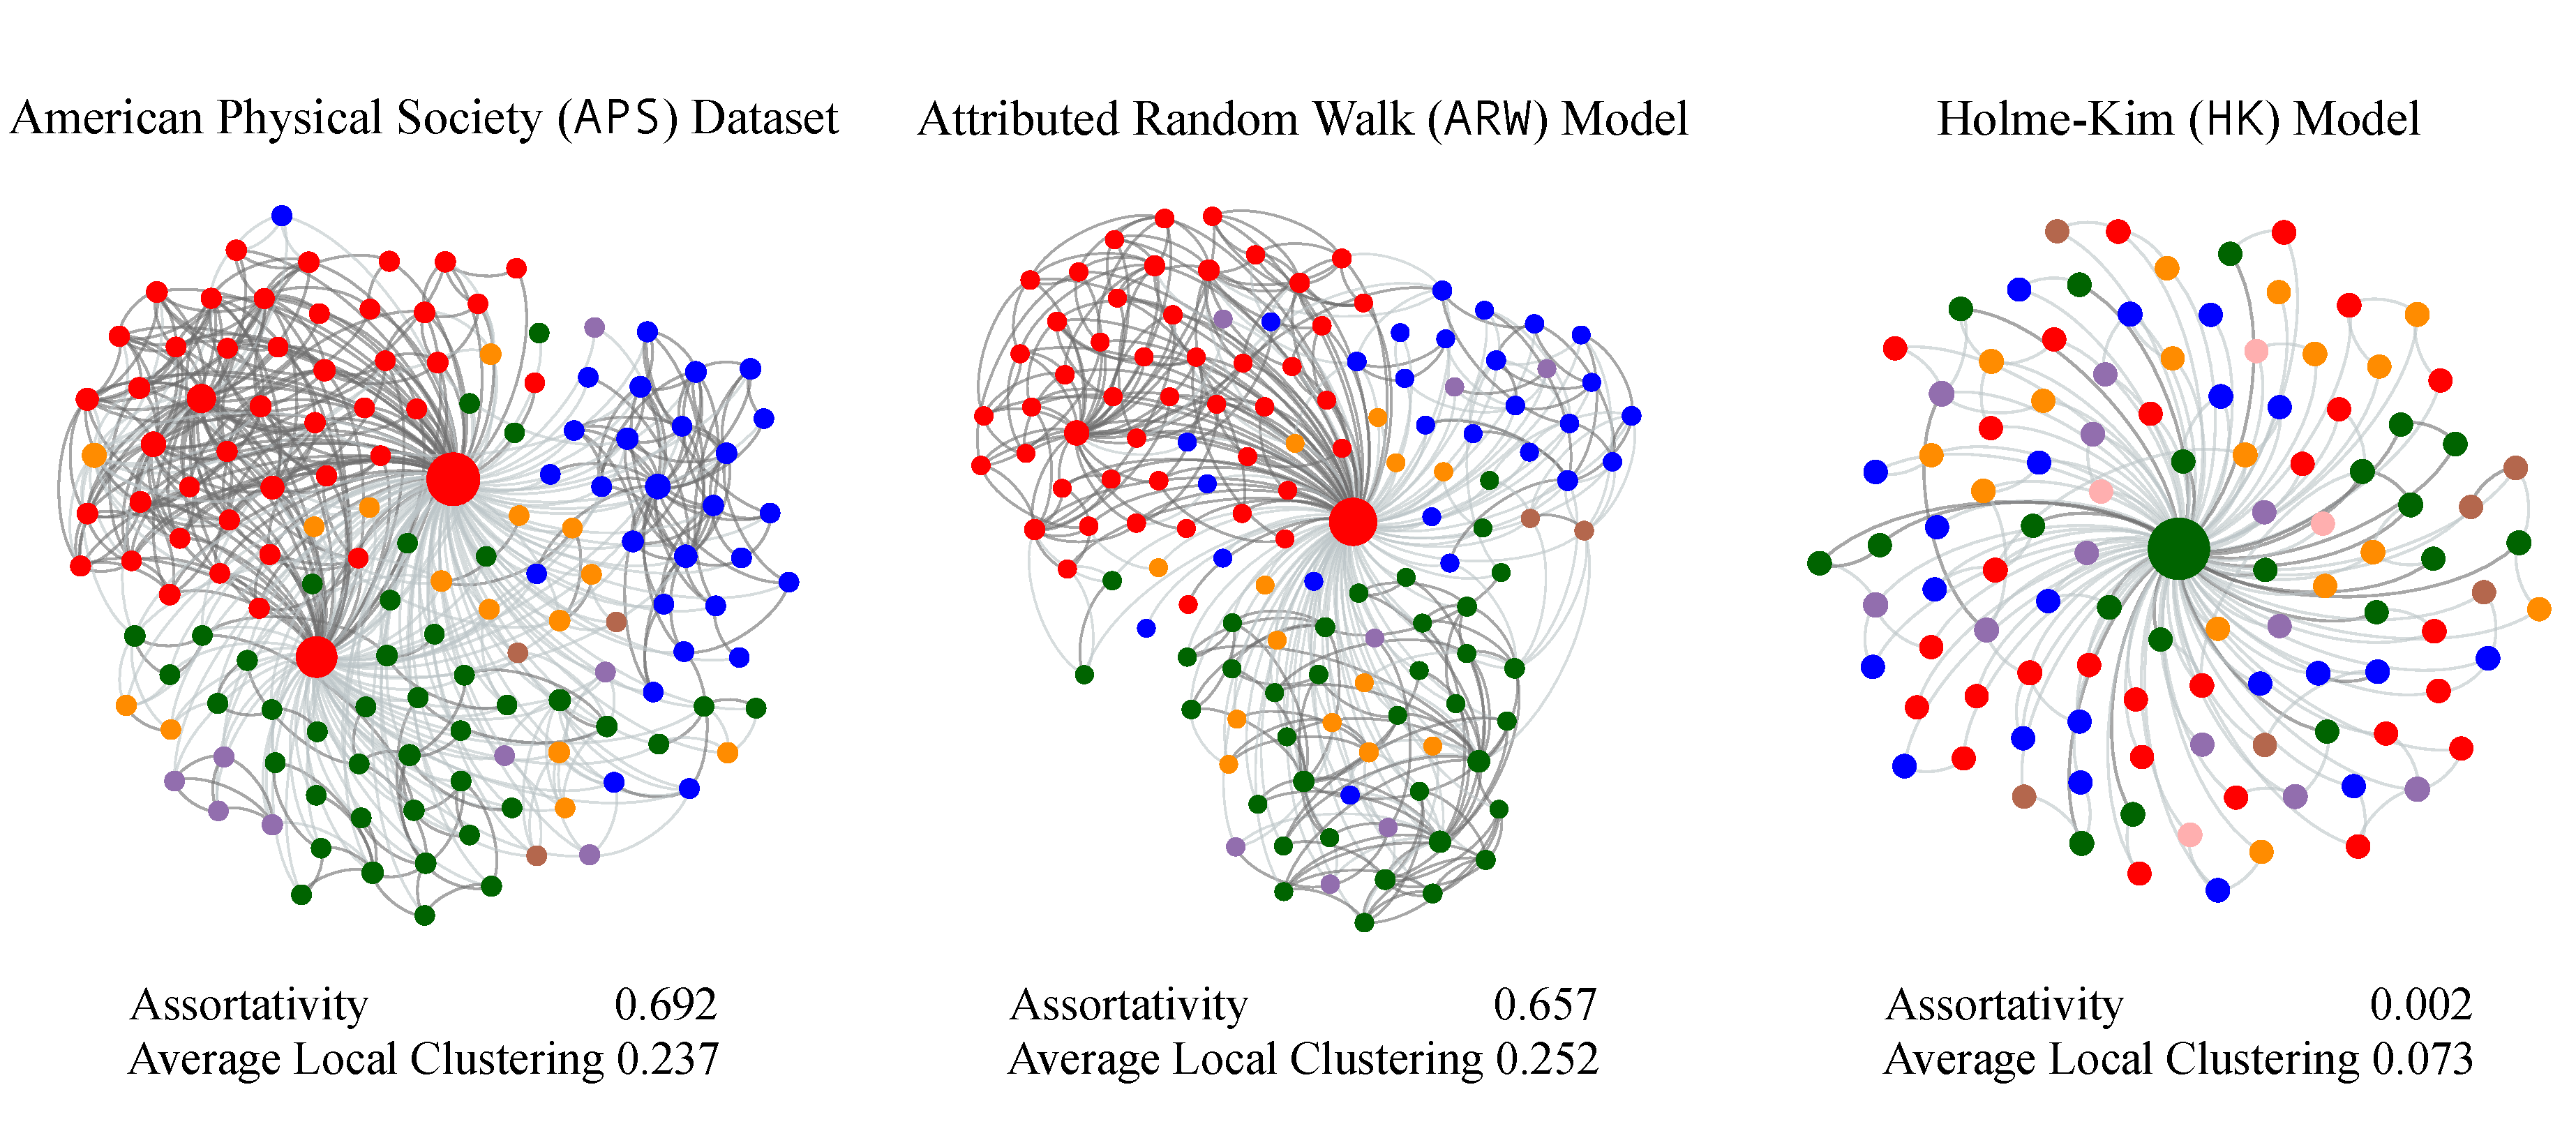
\includegraphics[width=\columnwidth]{experiments_final4}
    \vspace{1pt}
    \caption{The figure shows how our proposed model of an Attributed Random Walk (\texttt{ARW}) accurately preserves local clustering and assortativity; we contrast with a non-attributed growth model~\cite{holme2002growing} to underscore the importance of using attributes for network growth.}
	\label{fig:intro_plot}
\end{figure}


We propose an Attributed Random Walk (\texttt{ARW}) model that jointly explains
the emergence of in-degree distributions, local clustering, clustering-degree
relationship and attribute mixing patterns through a resource constrained mechanism based on random walks (see~\Cref{fig:intro_plot}). In particular, \texttt{ARW} relies entirely on local information to grow the network, without access to information of all nodes. In \texttt{ARW}, incoming nodes select a seed node based on attribute similarity and initiate a biased random walk: at each step of the walk, the incoming node either jumps back to its seed or chooses an outgoing link or incoming link to visit another node; it links to each visited node with some probability and halts after it has exhausted its budget to form connections. We have three primary contributions:
\begin{enumerate}
\item \textbf{Attributed:} We propose a parsimonious and accurate model of attributed network growth.
\item \textbf{Local information:} Our model is based on a random walk and uses local processes to form edges, without recourse to global information of the network.
\item \textbf{Unified account:} To the best of our knowledge, \texttt{ARW} is the first model that accounts for multiple sociological phenomena---bounded rationality; structural constraints; triadic closure; attribute homophily; preferential attachment---through an entirely local process to model global network structure and attribute mixing patterns.
\end{enumerate}



% We conducted extensive experimental results against state-of-the-art
% baselines on large and diverse citation network datasets.
% We focus on directed citation networks
%  in this paper, as these networks---where all node edges form at the time of node joining---offer a clean foundation to explain growth in social networks (e.g. via a ``pause \& restart'' parameter), where edges can form after a node joins.
\texttt{ARW} preserves multiple structural properties---in-degree distribution, clustering and
indegree-clustering relationship---with high accuracy.
Our experiments on six large-scale network datasets indicate that the proposed growth model outperforms
eight state-of-the-art network growth models, including attributed growth models, by a
statistically significant margin of 2.5--$10\times$.

The rest of the paper is organized as follows.
We begin by defining the problem statement in~\Cref{sec:Problem Statement}.
In~\Cref{sec:Analysis}, we outline six network datasets, describe key structural
properties of real-world networks and discuss insights from sociological studies.
Then, in~\Cref{sec:Proposed Model}, we describe the network growth model. We follow
by presenting experiments in ~\Cref{sec:Experiments}, analysis of assortative mixing
in ~\Cref{subsec:LocalMixing} and discussion in~\Cref{sec:Discussion}.
We conclude in~\Cref{sec:Conclusion}.
%!TEX root = ../main.tex

\section{Problem Statement}
\label{sec:Problem Statement}

Consider an attributed directed network $G=(V,E,B)$, where $V$ \& $E$ are
sets of nodes \& edges and each node has an attribute value $b \in B$.
The goal is to develop a directed network growth model that preserves structural
and attribute based properties observed in $G$. The growth model should be
normative, accurate and parsimonious:
\begin{enumerate}
\item \textbf{Normative}: The model should account for multiple sociological phenomena that influence how individuals form edges under constraints of limited global information and partial network access.

\item \textbf{Accurate}: The model should preserve key structural
and attribute based properties: degree distribution,
local clustering, degree-clustering relationship and attribute mixing patterns.

\item \textbf{Parsimonious}: The model should be able to
generate networks with tunable structural properties, while having few parameters.
\end{enumerate}
% \begin{enumerate}
%     \item \textbf{Normative}: The model should account for multiple sociological phenomena that influence how individuals form edges under
%     constraints of limited global information and partial network access.
%     \item \textbf{Accurate}: The model should preserve key structural
%     and attribute based properties: degree distribution,
%     local clustering, degree-clustering relationship and attribute mixing patterns.
%     \item \textbf{Parsimonious}: The model should be expressive enough to
%     generate networks with tunable structural properties, while having as few parameters as possible.
% \end{enumerate}

Next, we present empirical analysis on real-world datasets to motivate our attributed random walk model.

% \clearpage
%!TEX root = draft.tex

\section{Empirical Analysis}
\label{sec:Analysis}

In this section, we begin by describing six large-scale network datasets that we use in our
analysis and experiments. Then, we
describe key factors that impact edge formation and analyze global structural
properties of real-world networks. Finally, we briefly discuss insights from
empirical studies in sociology and common assumptions in network modeling.

\subsection{Datasets}
\label{sec:Datasets}

We consider six citation networks of different scales (size, time) from diverse
sources: research articles, utility patents and judicial cases. We list the
summary statistics and global network properties of these datasets in~\Cref{table:datasets}.
Three of the six datasets are attributed networks; That is, each node has a categorical attribute value.

We focus on citation networks for two reasons. First, since nodes in citation networks form
all outgoing edges to existing nodes at the time of joining the network,
citation networks provide a clean basis to study edge formation mechanisms in
attributed networks. Second, citation network span long periods of time (e.g.
the \texttt{USSC} judicial citation network span several hundred years).
Consequently, identifying local edge formation processes that successfully model
growth for this duration is non-trivial.
Next, we study the structural and content properties of these networks.

% Now, we briefly describe the datasets considered in this paper.
% \Cref{table:datasets} provides summary statistics of the following networks:
% \begin{enumerate}
%     % (V,E) = (22049, 138871), used (V,E): 18665 115358
%     \item{\textbf{Association of Computational Linguistics}} (\texttt{ACL}) \cite{acldata} is an attributed academic citation network
%     that consists of papers published in ACL conferences, journals and workshops.
%     The attribute value of each paper is the name of the venue where it was published.
%
%     % (V,E) = (22049, 138871), used (V,E): 18665 115358
%     % \item{\textbf{Python Package Index}} (\texttt{PYPI}) \footnote{http://web.stanford.edu/class/cs224w/resources.html} is an attributed dependency graph of Python
%     % software packages. Each software package is associated with a category.
%
%     % entire dataset used
%     \item{\textbf{U.S. Supreme Court Cases}} (\texttt{USSC}) \cite{fowler2008authority} is a judicial citation network of
%     U.S. Supreme Court cases. There is an edge from case $i$ to case $j$ if and only if case $i$ cites case $j$ in its majority opinion.
%
%     % used: (V,E) = (30,558, 347,228) after removing nodes w. missing time data
%     \item{\textbf{ArXiv HEP-PH}} (\texttt{HEP-PH}) \cite{gehrke2003overview} is an academic citation network of HEP-PH (high energy
%     physics phenomenology) papers in the ArXiv e-print.
%
%     % used: (V,E) = (556661, 6647769) after removing nodes w. missing time + categorial data
%     \item{\textbf{APS Journals}} (\texttt{APS}) is an attributed academic citation network maintained by
%     the American Physical Society (\texttt{APS}).
%     The attribute value of each paper is the \texttt{APS} journal in which it was published.
%
%     % used: (V,E) = (2047881, 10088564) after removing nodes w. missing time + categorical data
%     \item{\textbf{U.S Utility Patents}} (\texttt{Patents}) \cite{leskovec2005graphs} is an attributed citation network of U.S. utility patents maintained by
%     the National Bureau of Economic Research (NBER).
%     The attribute value of each patent is an NBER patent category.
%
%     % used: (V,E) = (5987642, 45028807) after removing nodes w. missing time data
%     \item{\textbf{Semantic Scholar}} (\texttt{Semantic}) \cite{ammar} is an academic citation network of
%     Computer Science and Neuroscience papers, released in June 2017 by Semantic Scholar.
% \end{enumerate}

% in \cref{subsec:factors} and empirically
% validate the effectiveness of the proposed model using these network datasets in~\Cref{sec:Experiments}.
%
% In this section, we outlined the citation network datasets that we use in our analysis and experiments.
% Next, we discuss common factors that affect edge formation mechanisms and identify common global structural
% properties of real networks.


\subsection{Observations from Network Data}
\label{subsec:factors}

% Factors that influence edge formation at the nodal level have a cumulative
% effect on global structural properties of real-world networks.
Compact
statistical descriptors of global network properties ~\cite{newman2010networks}
such as degree distribution, local clustering and attribute assortativity
quantify the extent to which local edge formation phenomena shape global network
structure.

\textbf{Heavy tailed degree distribution:} All networks in~\Cref{table:netstats} exhibit heavy tailed degree distributions. These
distributions can arise out of the well known preferential attachment process~\cite{simon1955class,barabasi1999emergence}, where incoming nodes connect with nodes in proportion to their degree. As a result, initial differences in node
degree get reinforced over time, giving rise to heavy
tailed degree distributions.
% (also known as the ``rich get richer'' effect) in citation networks; It also implies that most papers receive zero or a few
% citations, but a small but significant percent of the nodes turn into popular
% hubs that receive many citations.
Log-normal fits, with parameters listed in ~\cref{table:netstats}, describe the in-degree
distribution of all network datasets, well consistent with~\citet{broido2018scale} observation that real-world networks with truly power law
degree distributions are rare.
% Our model explains the emergence of heavy tailed in-degree distributions through a \textit{local} process that adjusts bias towards linking to well-connected nodes

\begin{figure}[H]
 \vspace{-10pt}
 \centering
 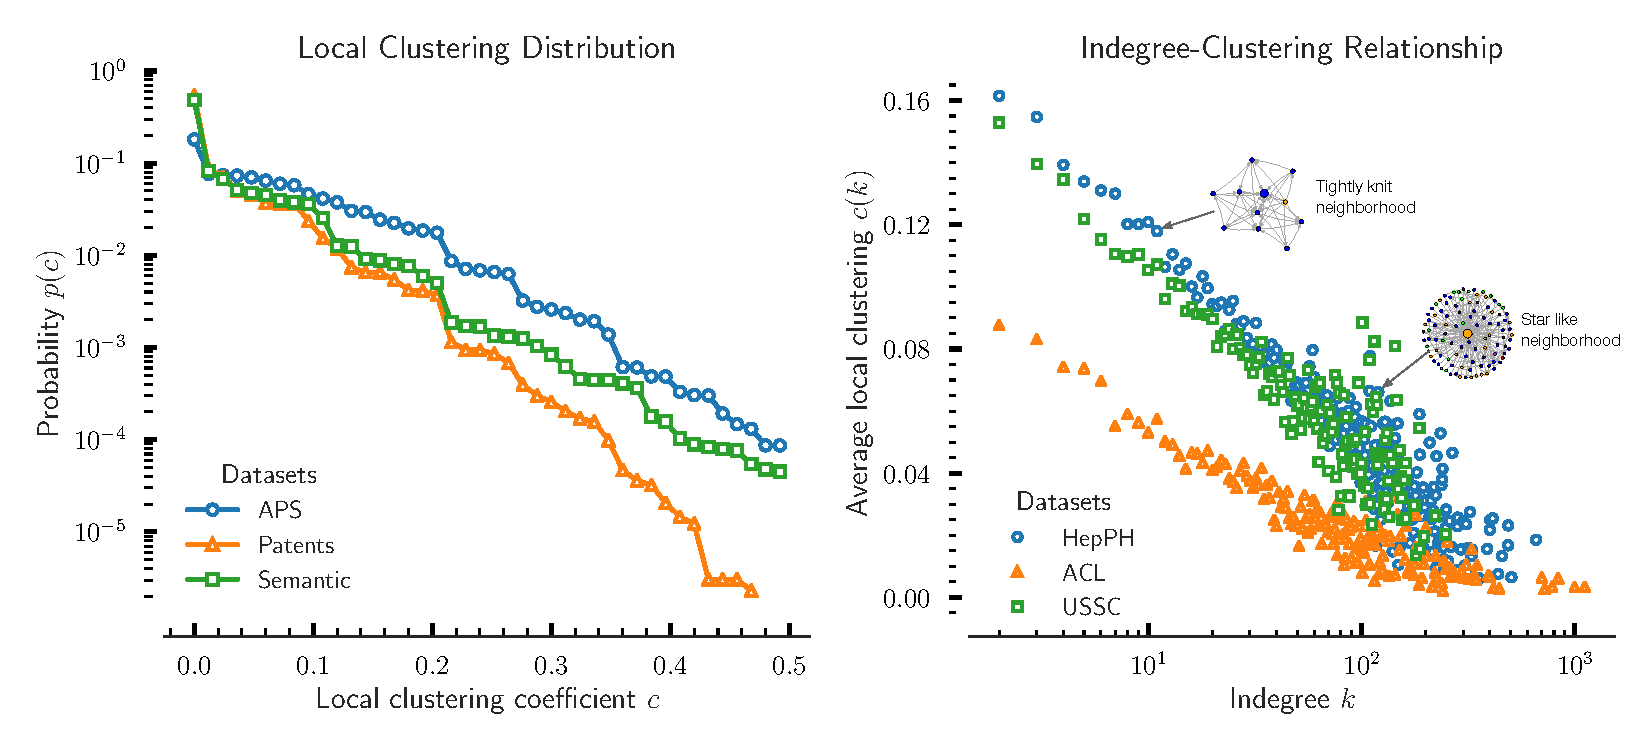
\includegraphics[width=.9\columnwidth]{cc_analysis2}
 \caption{
    Local clustering in real-world networks have common characteristics:
    skewed local clustering distribution (left subplot) and a negatively correlated
    relationship between in-degree and average local clustering (right subplot).
 }
 \label{fig:cc_dc}
 \vspace{-10pt}
\end{figure}

\textbf{High Local Clustering:} Real-world networks tend to exhibit high average local clustering, as shown in~\Cref{table:netstats}. We can explain local clustering due to the phenomena of triadic closure~\cite{simmel1950sociology,
newman2001clustering}, where nodes with common neighbor(s) have an increased
likelihood of forming a connection.
% Empirical studies
% \cite{kossinets2006empirical} show that the probability of edge formation
% increases with the number of common neighbors.
The local clustering coefficient of a node measures the prevalence of triadic closure in its neighborhood; It is the probability that two randomly chosen neighbors of the node $i$ are connected. In directed networks, the neighborhood of a node $i$ can refer to the
set of nodes that link to $i$, set of nodes that $i$ links to or the union of
both sets. We define the neighborhood to be the set of all nodes that link to
node $i$.  However, average local clustering is not a
representative statistic of the \textit{skewed} local clustering distributions
shown in~\Cref{fig:cc_dc}. Furthermore, real-world networks exhibit a negative
correlation between node in-degree  and local clustering. As shown in~\Cref{fig:cc_dc}, the average local clustering  decreases as in-degree increases.
That is, low in-degree nodes have small, tightly knit neighborhoods and high
in-degree nodes tend have large, star-shaped neighborhoods.

% We propose a model
% that explains how clustering in real-world networks can arise from local processes
% of exploration \& link formation.


% Homophily and Assortativity
\textbf{Homophily:}
Real-world attributed networks exhibit homophily~\cite{mcpherson2001birds}, the phenomenon where similar nodes are more likely
to be connected than dissimilar nodes. The assortativity coefficient
~\cite{newman2002assortative} $r \in [-1, 1]$,
% defined as the ratio between the observed modularity and
% the maximum possible modularity with respect to set of attribute values $B=\{b_1...b_l\}$,
quantifies the level of homophily in an attributed network. Intuitively, it
compares the observed fraction of edges between nodes with the same attribute
value to the expected fraction of edges between nodes with same attribute value
if the edges were rewired randomly.
Attributed networks \texttt{ACL}, \texttt{APS} \& \texttt{Patents} exhibit
varying level of homophily, as shown in~\Cref{fig:mixing}, with assortativity
coefficient ranging from $0.07$ to $0.72$.
The magnitude of the attribute assortativity
signifies the extent to which attribute similarity influences edge formation.

% We embed attribute based preferences at the local level lead to generate networks
% with varying attribute mixing patterns.

\begin{figure}
 \centering
 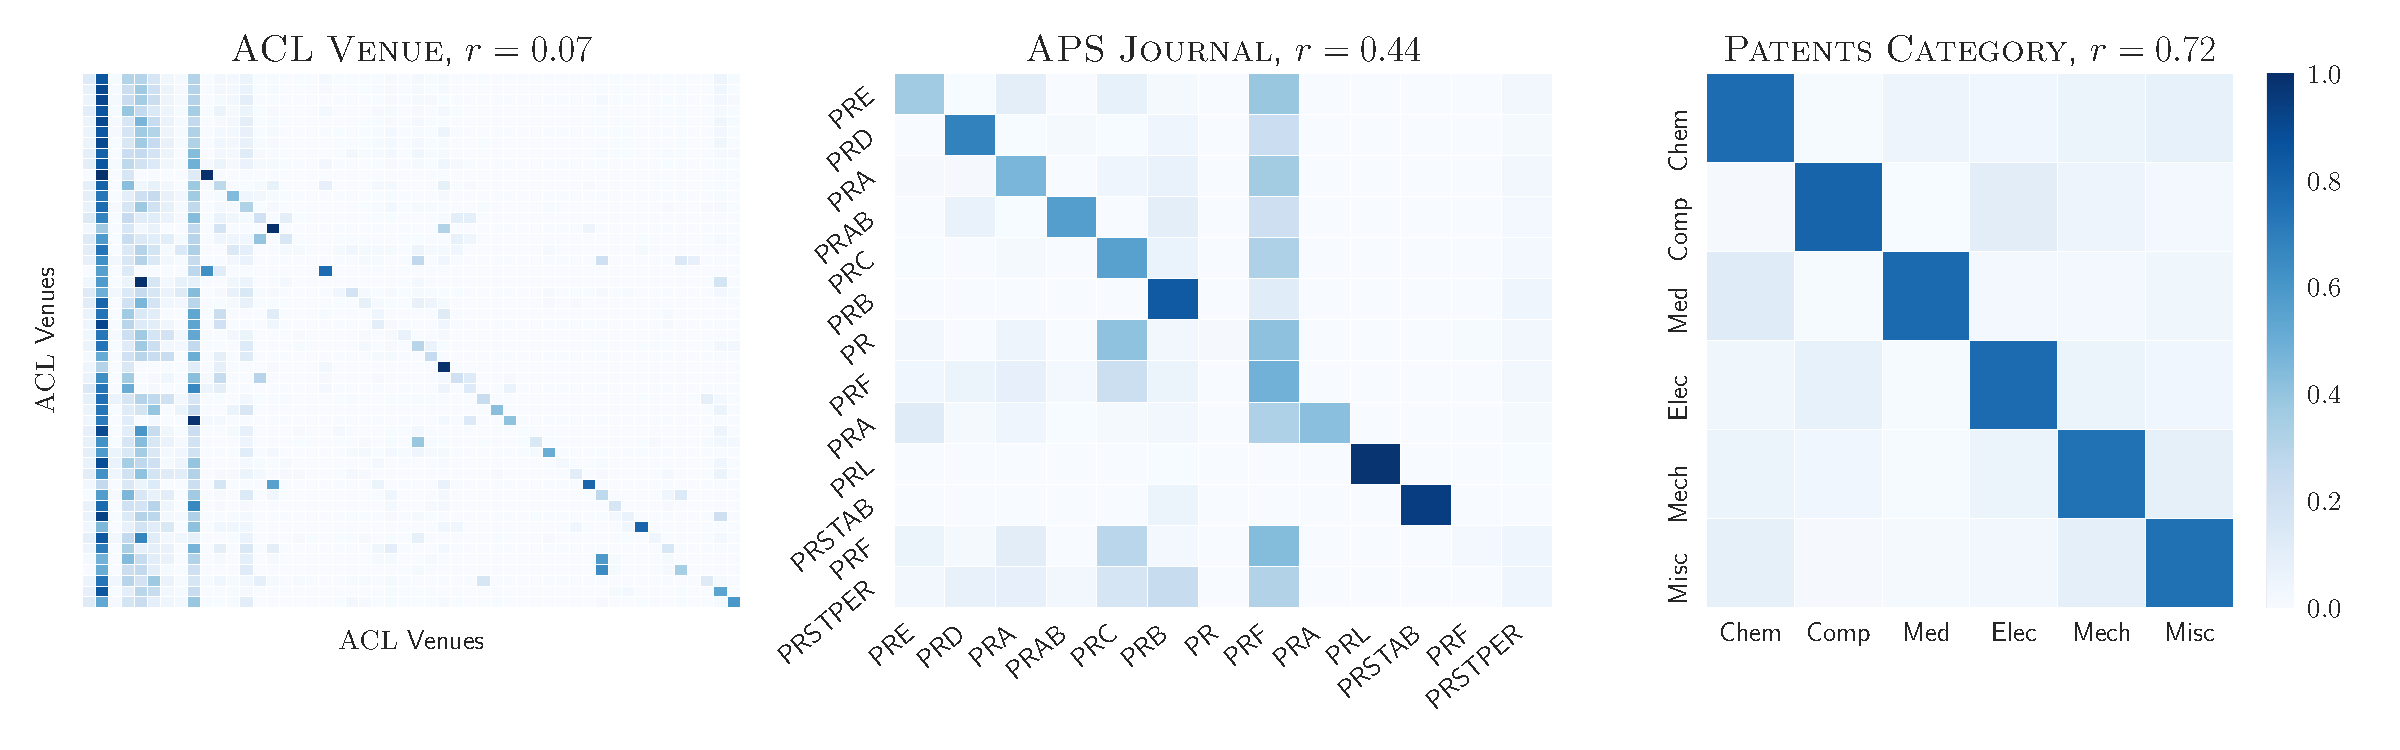
\includegraphics[width=\columnwidth]{mixing_v3}
 \caption{
    Attributed networks exhibit varying levels of homophily. The subplots
    illustrate the mixing patterns in \texttt{ACL}, \texttt{APS} and \texttt{Patents}
    w.r.t. attributes \texttt{Venue} ($r=0.07$), \texttt{Journal} ($r=0.44$) and
    \texttt{Category} ($r=0.72$) respectively.
 }
 \label{fig:mixing}
 \vspace{-25pt}
\end{figure}

\textbf{Increasing Out-degree over Time:}
The out-degree of nodes that join real-world networks tends to increase
as functions of network size and time. This phenomenon densifies networks and shrinks their
diameter over time. Densification tends to exhibit a power law relationship
~\cite{leskovec2005graphs} between the number of edges $e(t)$ and nodes $n(t)$ at time $t$: $e(t) \propto n(t)^{\alpha}$.~\Cref{table:netstats} lists the densification power law exponent $\alpha$ of the network datasets.

To summarize, citation networks tend to be homophilic networks that undergo
accelerated network growth and exhibit regularities in structural properties:
heavy tailed in-degree distribution, skewed local clustering distribution,
negatively correlated degree-clustering relationship and varying attribute
mixing patterns.

% In our proposed model, we increase the outdegree of incoming nodes at a linear or superlinear rate to account for the accelerated network growth observed in real networks.

% To summarize, factors such as preferential attachment, triadic closure and homophily not only effect how individuals form connections at the local level but also explain regularities arise in global structural properties of real-world networks. Next, we discuss empirical studies from sociology that examine network formation and decision making.

\subsection{Insights from Sociological Studies}

Sociological studies on network formation seek to explain
how individuals form edges in real-world networks.

\textbf{Interplay of Triadic Closure and Homophily:} Empirical studies~\cite{35626,block2014multidimensional} that investigate
the interplay between triadic closure and homophily in evolving networks
indicate that \textit{both} structural proximity and homophily are statistically
significant factors that simultaneously influence edge formation. While homophilic preferences~\cite{mcpherson2001birds} induce edges between similar nodes, structural factors (e.g. network distance) act as constraints that restrict edge formation to structurally proximate nodes (e.g. friend of a friend).

\textbf{Bounded Rationality:} Extensive work~\cite{simon1972theories,gigerenzer1996reasoning,lipman1995information}
on individual decision making indicates that individuals are \textit{boundedly}
rational actors. That is, individuals make decisions under constraints of limited information, cognitive capacity and time. This implies that individuals that join networks employ simple rules to form edges under constraints of limited information and partial network access. For example, a researcher cites academic papers without knowledge of or access
to the entire literature in her or his field.

Current preferential attachment and fitness-based models
\cite{dorogovtsev2000structure,kim2017effect,singh2017relay,barabasi1999emergence} make two assumptions that are at variance with these findings in the Social Sciences. First, by assuming that successive edge formations are independent, these models disregard the effect of triadic closure and structural proximity. Second, they implicitly require incoming nodes to have complete network access (e.g., be able to connect to any node) or explicit knowledge of one or more properties (e.g., fitness, degree) of \textit{every} node in the network. For example, a preferential attachment model, by making connections in proportion to degree, requires \textit{non-local} information: the degree distribution of the entire network.

To summarize, insights from the social sciences suggest that edge formation in real-world networks is biased towards nodes that are similar, proximate or well-connected and that
these edges are made under constraints of limited information and network access.
The global properties described in~\cref{subsec:factors} are modulated by the presence of
resource constrained edge formation decisions.

Next, we propose a growth model that uses \textit{local} processes for
edge formation and which lead to the emergence of global structural and attribute properties observed in real-world networks.

% citation networks tend to be homophilic networks that
% undergo accelerated network growth and exhibit regularities in structural
% properties: heavy tailed in-degree distribution, skewed local clustering distribution, negatively correlated degree-clustering relationship and varying attribute mixing patterns. These global properties are modulated by the presence of resource constrained edge formation decisions.


% and global structural properties can be better understood by studying network snapshots at different stages of the growth process.


% datasets include the time (e.g., publication year of academic papers) at which nodes join the network. As a result, local edge formation processes and global structural properties can be better understood by studying network snapshots at different stages of the growth process. Third, the citation networks are large networks that tend to have one or more nodal attributes (e.g. category of patents)
% and span multiple decades. As a result, the structural and content properties of the citation
% networks considered are well-defined.

% Nodes do
% not form or delete edges at a later time. This allows us to analyze
% the edge formation mechanisms of new nodes that join the network form edges.
% % Other edge dynamics such as edge deletion and addition of edges between existing
% % nodes are important and we plan to investigate them at a later time.
% Second, citation network datasets include the time (e.g., publication year of academic
% papers) at which nodes join the network. As a result, local edge formation
% processes and global structural properties can be better understood by studying
% network snapshots at different stages of the growth process. Third, the citation
% networks are large networks that tend to have one or more nodal attributes (e.g. category of patents)
% and span multiple decades. As a result, the structural and content properties of the citation
% networks considered are well-defined.

% \begin{table}[b]
%  \center
%  {
%   \begin{tabular}[c]{lrrrr} \toprule
%   Network Dataset &  \texttt{LN} $(\mu, \sigma)$ & \texttt{DPL} $\alpha$       &  Avg. ${\texttt{LCC}}$  & \texttt{AA} $r$   \\ \midrule
%   \texttt{USSC}     &   (1.19, 1.18) & 2.32     & 0.12    & -     \\
%   \texttt{HEP-PH}   &   (1.32, 1.41) & 1.67     & 0.12    & -     \\
%   \texttt{Semantic} &   (1.78, 0.96)  & 1.58     & 0.06    & -     \\   \midrule
%   \texttt{ACL}      &   (1.93, 1.38)  & 1.43     & 0.07    & 0.07     \\
%   \texttt{APS}      &   (1.62, 1.20)  & 1.26     & 0.11    & 0.44     \\
%   \texttt{Patents}  &   (1.10, 1.01)   & 1.94     & 0.04    & 0.72    \\
%   % \texttt{PYPI}         & 1.208     & 0.0524    & 0.692   & a\\
%    \bottomrule
%   \end{tabular}
%   \vspace{1mm}
%   \caption{Global network properties: lognormal (\texttt{LN}) in-degree distribution mean and standard deviation $(\mu, \sigma)$,
%   densification power law (\texttt{DPL}) exponent $\alpha$, average local clustering coefficient (${\texttt{LCC}}$)
%   and attribute assortativity (\texttt{AA}) coefficient of six network datasets.}
%   \label{table:netstats}
%  }
% \end{table}


% \clearpage
%!TEX root = draft.tex
\vspace{-6pt}
\section{Attributed Random Walk Model}
\label{sec:Proposed Model}
We propose an Attributed Random Walk (\texttt{ARW}) model to explain the emergence
of key structural properties of real-world networks through \textit{entirely local}
edge formation mechanisms.

Consider a stylized example of how a researcher might go about finding relevant papers to cite. First, the researcher broadly identifies one or more \textit{relevant} papers,
possibly with the help of external information sources (e.g. Google Scholar). These initial set of papers act as seed nodes.  Then, acting under time and information constraints, she will examine papers that cite a seed paper, as well as those papers cited by the seed. Thus she navigates a chain of references to identify \textit{similar} papers relevant to addressing that research question in which she is interested. Next, through careful analysis, she will cite a subset of these papers.

\texttt{ARW} grows a directed network as new nodes join the network. The
mechanism is motivated by the stylized example: an incoming node selects a seed node and initiates a random walk to explore the network by navigating through neighborhoods of existing nodes. It halts the random walk after connecting to a few visited nodes.

In this section, we describe the edge formation mechanisms underlying
\texttt{ARW} and explain how \texttt{ARW} provides a unified treatment of
the observations from empirical data as well as Social Science studies. Then,
we discuss the methods required to fit \texttt{ARW} to data.

% intuitively incorporates multiple sociological phenomena.

\subsection{Model Details}
\label{sub:Model Description}


The Attributed Random Walk (\texttt{ARW}) model grows a directed network $\{\hat{G}_t\}^T_{t=1}$
in $T$ time steps.
More formally, at every discrete time step $t$, a
new node $u$, with attribute value $B(u)$, joins the network $\hat{G}_t$.
After joining the network, node $u$ forms $m(t)$ edges to
existing nodes.
% At time $t$, $G_t$ consists of ${|V_t|=|V_0|+t}$ nodes,
% ${|E_t|=|E_{t-1}|+m(t)}$ edges and the set of attribute values ${A_t = A_{t-1}
% \cup \{A(u)\}}$.
The out-degree of incoming nodes increases over time to
reflect the nonlinear growth and densification of real-world networks.
% We discuss the
% issue of initializing $G_0$, sampling attribute values of inomcing nodes and modeling
% densification in \Cref{sub:Model Fitting}.

The edge formation mechanism consists of two components: \textsc{Select-Seed} and
\textsc{Random-Walk}. An incoming node $u$ with attribute value $B(u)$ that joins the
network at time $t$ first selects a seed node $S(u)$ using \textsc{Select-Seed}:
\\\\
\tikzstyle{background rectangle}=[thin,draw=black]
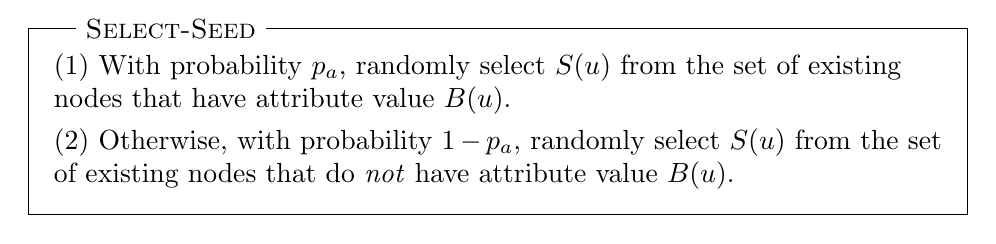
\begin{tikzpicture}[show background rectangle]
	\node[align=left, text width=.93\linewidth, inner sep=.5em]{
		(1) With probability $p_a$, randomly select $S(u)$ from the set of existing nodes that have attribute
		value $B(u)$.

		\vspace{1mm}
		(2) Otherwise, with probability $1-p_a$, randomly select $S(u)$ from the set of existing nodes that
		do \textit{not} have attribute value $B(u)$.
	};
	\node[xshift=3ex, yshift=-.7ex, overlay, fill=white, draw=white, above
	right] at (current bounding box.north west) {
		\textsc{Select-Seed}
	};
\end{tikzpicture}

% The attribute parameter $p_a$ incorporates the attribute preferences of incoming nodes
% into the model.

\textsc{Seed-Select} accounts for homophilic preferences of incoming nodes using
attribute parameter $p_a$. As shown in \cref{fig:randomwalk}, after selecting
the seed $S(u)$, node $u$ initiates a
random walk using \textsc{Random-Walk} to form $m(t)$ links.
The \textsc{Random-Walk} mechanism consists of four parameters: the rate parameter $\alpha$
\& attribute parameter $p_a$ model edge formation decisions and the jump parameter $p_j$ \&
outlink parameter $p_o$ characterize random walk traversals:
\\\\
\tikzstyle{background rectangle}=[thin,draw=black]
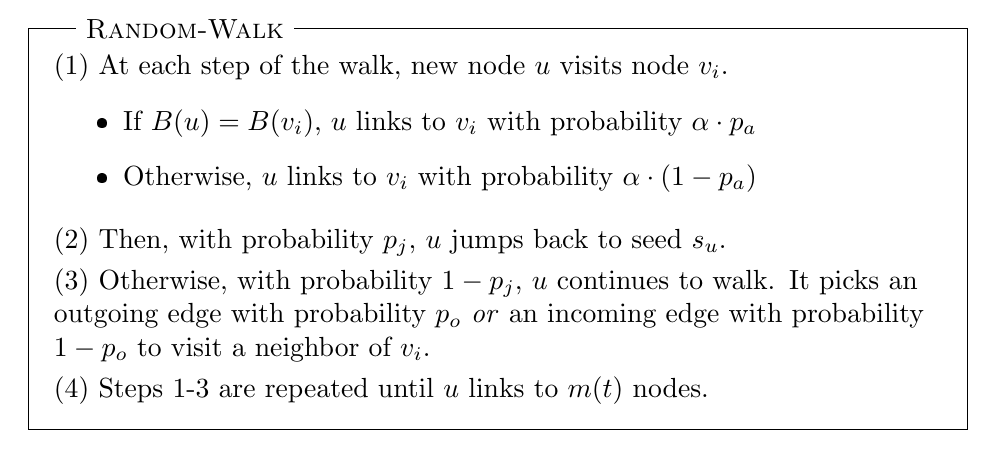
\begin{tikzpicture}[show background rectangle]
	\node[align=left, text width=.93\linewidth, inner sep=.5em]{
		(1) At each step of the walk, new node $u$ visits node $v_i$.
		\begin{itemize}
			\item If $B(u)=B(v_i)$, $u$ links to $v_i$ with probability $\alpha \cdot p_a$
			\item Otherwise, $u$ links to $v_i$ with probability $\alpha \cdot (1-p_a)$
		\end{itemize}

		\vspace{1mm}
		(2) Then, with probability $p_j$, $u$ jumps back to seed $s_u$.

		\vspace{1mm}
		(3) Otherwise, with probability ${1-p_j}$, $u$ continues to walk. It picks an outgoing edge with probability $p_o$ \textit{or}
		an incoming edge with probability $1-p_o$ to visit a neighbor of $v_i$.

		\vspace{1mm}
		(4) Steps 1-3 are repeated until $u$ links to $m(t)$ nodes.
	};
	\node[xshift=3ex, yshift=-.7ex, overlay, fill=white, draw=white, above
	right] at (current bounding box.north west) {
		\textsc{Random-Walk}
	};
\end{tikzpicture}

When attribute data is absent, the attribute parameter $p_a$ is not required.
Then, \textsc{Seed-Select} simply selects an existing node uniformly at random
and the probability of edge formation in \textsc{Random-Walk} is equal to
the rate parameter $\alpha$ only.

Notice that \texttt{ARW} has two exogenous parameters:  the average out-degree $m(t)$ and attribute $B(u)$ of the node joining the network. The parameter $m(t)$ is similar to the parameter $m$ in the classic Preferential-Attachment model~\cite{barabasi1999emergence}, except that $m(t)$ is the mean-field value of degree $m$ at time $t$. While it is straightforward to model $m(t)$ endogenously by incoporating a densification power-law \texttt{DPL} exponent $\alpha$ to \texttt{ARW}, we decided against it, since exogenous factors to may explain changes to $m(t)$. For example, the number of citations in a paper can be influenced by venue (e.g. \texttt{WSDM2019} allows for one page of references); also, our empirical data analysis shows that papers early in a citation network tend to have few citations on average, perhaps explained by availability of \textit{fewer} papers to cite. The attribute distribution $B(u)$ varies with time as new journals or venues crop up, necessitating an exogenous parameter.



Next, we explain how each parameter is necessary to conform to normative
behavior of individuals in evolving networks.

\begin{figure*}
	\vspace{-20pt}
    \centering
    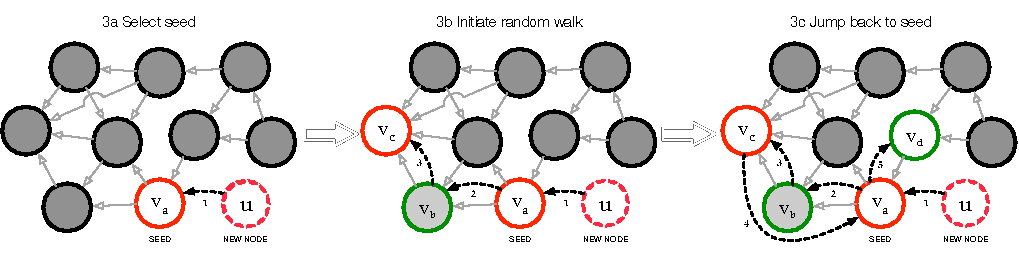
\includegraphics[width=.9\linewidth]{rw_diag2}
    \caption{Edge formation in \texttt{ARW}: consider
    an incoming node $u$ with outdegree ${m=3}$ and attribute value {$B(u)=\textsc{red} \in \{\textsc{red},\textsc{green}\}$}.
    In fig. 3a, $u$ joins the network and selects seed $v_a$ via \textsc{Select-Seed}.
    Then, in fig. 3b, $u$ initiates a \textsc{Random-Walk} and traverses from $v_a$ to $v_b$ to $v_c$.
    Finally, $u$ jumps back to its seed $v_a$ and restarts the walk, as shown in fig. 3c.
    Node $u$ halts the random walk after linking to $v_a$, $v_c$ \& $v_d$.
    }
    \label{fig:randomwalk}
	\vspace{-8pt}
\end{figure*}


\subsection{\texttt{ARW} and Normative Behavior}
\label{sub:Model Interpretation}

The Attributed Random Walk model unifies multiple sociological phenomena
into its edge formation mechanisms.

\newtheoremstyle{exampstyle}
  {2pt} % Space above
  {2pt} % Space below
  {\itshape} % Body font
  {} % Indent amount
  {\bfseries} % Theorem head font
  {.} % Punctuation after theorem head
  {.25em} % Space after theorem head
  {} % Theorem head spec (can be left empty, meaning `normal')

\theoremstyle{exampstyle} \newtheorem{ph}{Phenomenon}

\begin{ph}
	(Limited Resources) Individuals are boundedly rational~\cite{simon1972theories,gigerenzer1996reasoning,lipman1995information}
	actors that form edges under constraints of limited information, partial network access and finite cognitive capacity.
\end{ph}
\texttt{ARW} uses a random walk to incorporate constraints of limited information
and partial network access. A new node $u$ selects a seed node from which it
initiates a biased random walk. Then, $u$ uses simple rules to connect to each visited
nodes probabilistically and halts the walk after forming $m(t)$ edges, as shown in~\Cref{fig:randomwalk}. Random walks require information only about the
1-hop neighborhood of visited nodes, thus accounting for  the constraints of limited information and partial network access.

\begin{ph}
	(Structural Constraints) Structural factors such as network distance
	act as constraints that limit edge formation to proximate nodes.  \cite{35626}
\end{ph}

We incorporate structural constraints into \texttt{ARW} using the jump parameter $p_j$.
The jump parameter $p_j$ is the probability with which a new node jumps back to its seed node
after each step of the random walk. This implies that the probability with which the new node
is at most $k$ steps from its seed node is $1-p^k_j$; As a result, the jump parameter $p_j$
controls the extent to which new nodes' random walks explore the network to form edges.

\begin{ph}
	(Triadic Closure) Nodes with common neighbors have an
	increased likelihood of forming a connection. \cite{simmel1950sociology}
\end{ph}

We control the effect of triadic closure on edge formation using the
rate parameter $\alpha$. A new node $u$ uses a random walk to
link to each visited node with probability proportional to $\alpha$. As a
result, the probability with which node $u$ closes a triad by linking to
a visited node and its neighbor is proportional to $\alpha^2$.

\begin{ph}
	(Attribute Homophily) Nodes that have similar attributes are more likely
	to form a connection. \cite{mcpherson2001birds}
\end{ph}
We incorporate attribute homophily into the edge formation process via attribute parameter $p_a$. New node
$u$ links to each visited node $v$ with probability $\alpha \cdot p_a$ if they share
the same attribute value. Otherwise, $u$ links with probability $\alpha \cdot (1-p_a)$.
The attribute parameter $p_a$ effectively controls global assortativity.

\begin{ph}
	(Preferential Attachment) Nodes tend to link to high degree nodes that have more
	visibility. \cite{barabasi1999emergence}
\end{ph}
% Individuals cannot link to high degree nodes \textit{directly} under constraints of limited information
% and partial network access.
\texttt{ARW} does not rely on global degree distribution. In absence of this global information, \texttt{ARW} can control the degree of preferential attachment by adding structural bias to the random walk traversals by varying the outlink probability $p_o$. Random walks that traverse outgoing edges only (i.e. $p_o =1$) eventually visit old nodes that tend to have high in-degree. Similarly, random walks that traverse incoming edges only (i.e. $p_o=0$) visit recently joined nodes that tend to have low indegree. We use parameter $p_o$, to adjust the effect of preferential attachment on edge formation.

To summarize: \texttt{ARW} incorporates five well-known sociological phenomena---bounded rationality; structural constraints; triadic closure; attribute homophily; preferential attachment---into a single edge
formation mechanism based on random walks.

% Random walks inherently account for
% limited information and partial network access. Furthermore, the jump parameter $p_j$, attribute parameter $p_a$,
% rate parameter $\alpha$ and out parameter $p_o$ incorporate the effect of structural constraints,
% homophily, triadic closure and preferential attachment respectively.



\subsection{Model Fitting}
\label{sub:Model Fitting}

We now briefly describe methods to estimate model parameters,
initialize $\hat{G}$, densify $\hat{G}$ over time and sample nodes' attribute values.

\textit{Parameter Estimation}.
% The rate parameter $\alpha$, attribute parameter $p_a$, jump parameter $p_j$ and
% out parameter $p_o$ jointly control the edge formation mechanism in \texttt{ARW}.
% These parameters subsequently determine the structural properties of the network $\hat{G}$
% generated by \texttt{ARW}.
The parameter estimation task consists of finding the set of
parameters values for $(\alpha, p_a, p_j, p_o)$ that best explain the structural properties
of an observed network $G$. We use a straightforward grid search method to estimate
the four parameters.
% Other derivative-free optimization methods such as the Nelder-Mead~\cite{nelder1965simplex}
% method can be used to speed-up parameter estimation.
% We describe the evaluation metrics and selection
% criteria in \Cref{sub:Experimental Setup}.

\textit{Initialization}. The edge formation mechanism in \texttt{ARW} is
sensitive to a large number of weakly connected components (\texttt{WCC}s) in the
initial network $\hat{G}_0$ because incoming nodes can only form edges to nodes
in the same \texttt{WCC}. To ensure that $\hat{G}_0$ is weakly
connected, we perform an undirected breadth-first search on the observed,
to-be-fitted network $G$ that starts from the oldest node and terminates after
visiting $0.1\%$ of the nodes. The initial network $\hat{G}_0$ is the small \texttt{WCC}
induced from the set of visited nodes.
% Simpler initialization methods
% such as sampling $\hat{G}_0$ from the Erdos-Renyi model or Watts-Strogatz model
% yield similar results.


\textit{Node Out-degree}.
% In \cref{sec:Analysis}, we observed that real
% networks densify over time, with the number of edges growing superlinearly in
% the number of nodes.
% To reflect the observation that the out-degree of incoming nodes increases over time in real-world networks, we do the following.
% We incorporate this phenomenon in \texttt{ARW}
% to coarsely reflect the rate of growth in the observed network $G$.
Each incoming node $u$ that joins $\hat{G}$ at time $t$ corresponds to some
node that joins the observed network $G$ in year $y(t)$; The number of edges $m(t)$
that $u$ forms is equal to the average out-degree of nodes that join $G$ in year $y(t)$.

\textit{Sampling Attribute Values}.
% In real networks $G=(V,E,B)$,
% the distribution over the set of attribute values $P_{\textsc{g}}(B)$ changes over time.
% For instance, the attribute distribution over journals in the \texttt{APS} citation
% network changes over time as old journals decay in popularity and new journals gain traction.
% The change in the attribute distribution over time is an exogenous factor and varies for every network.
% To incorporate this phenomenon into \texttt{ARW},
We sample the attribute value $B(u)$ of node $u$, that
joins $\hat{G}$ at time $t$, from $P_{\textsc{g}}(B{\mbox{ | year}=y(t)})$, the observed attribute distribution conditioned on the year of arrival of node $u$.

% \textit{Node -}.
% % In \cref{sec:Analysis}, we observed that real
% % networks densify over time, with the number of edges growing superlinearly in
% % the number of nodes.
% The - of incoming nodes increases over time in real-world networks.
% We incorporate this phenomenon in \texttt{ARW}
% to coarsely reflect the rate of growth in the observed network $G$.
% Each incoming node $u$ that joins $\hat{G}$ at time $t$ corresponds to some
% node that joins the observed network $G$ in year $y(t)$; The number of edges $m(t)$
% that $u$ forms is equal to the average - of nodes that join $G$ in year $y(t)$.

% \textit{Sampling Attribute Values}. In real networks $G=(V,E,B)$,
% the distribution over the set of attribute values $P_{\textsc{g}}(B)$ changes over time.
% For instance, the attribute distribution over journals in the \texttt{APS} citation
% network changes over time as old journals decay in popularity and new journals gain traction.
% The change in the attribute distribution over time is an exogenous factor and varies for every network.
% To incorporate this phenomenon into \texttt{ARW}, we sample the attribute value $B(u)$ of node $u$, that
% joins $\hat{G}$ at time $t$, from $P_{\textsc{g}}(B{\mbox{ | year}=y(t)})$, the observed attribute distribution
% conditioned on the corresponding year of node $u$.


To summarize, the \texttt{ARW} model
intuitively describes how individuals form edges under resource constraints.
\texttt{ARW} uses four parameters --- $\alpha$, $p_a$, $p_j$, $p_o$ --- to incorporate
individuals' biases towards similar, proximate and high degree nodes.
Next, our experiments in
\cref{sec:Experiments} show that $\texttt{ARW}$ accurately preserves
\textit{multiple} structural and attribute properties of real networks


% \clearpage
%!TEX root = ../main.tex

\begin{figure*}[t]
	\vspace{-15pt}
	\centering
	\makebox[\textwidth][c]{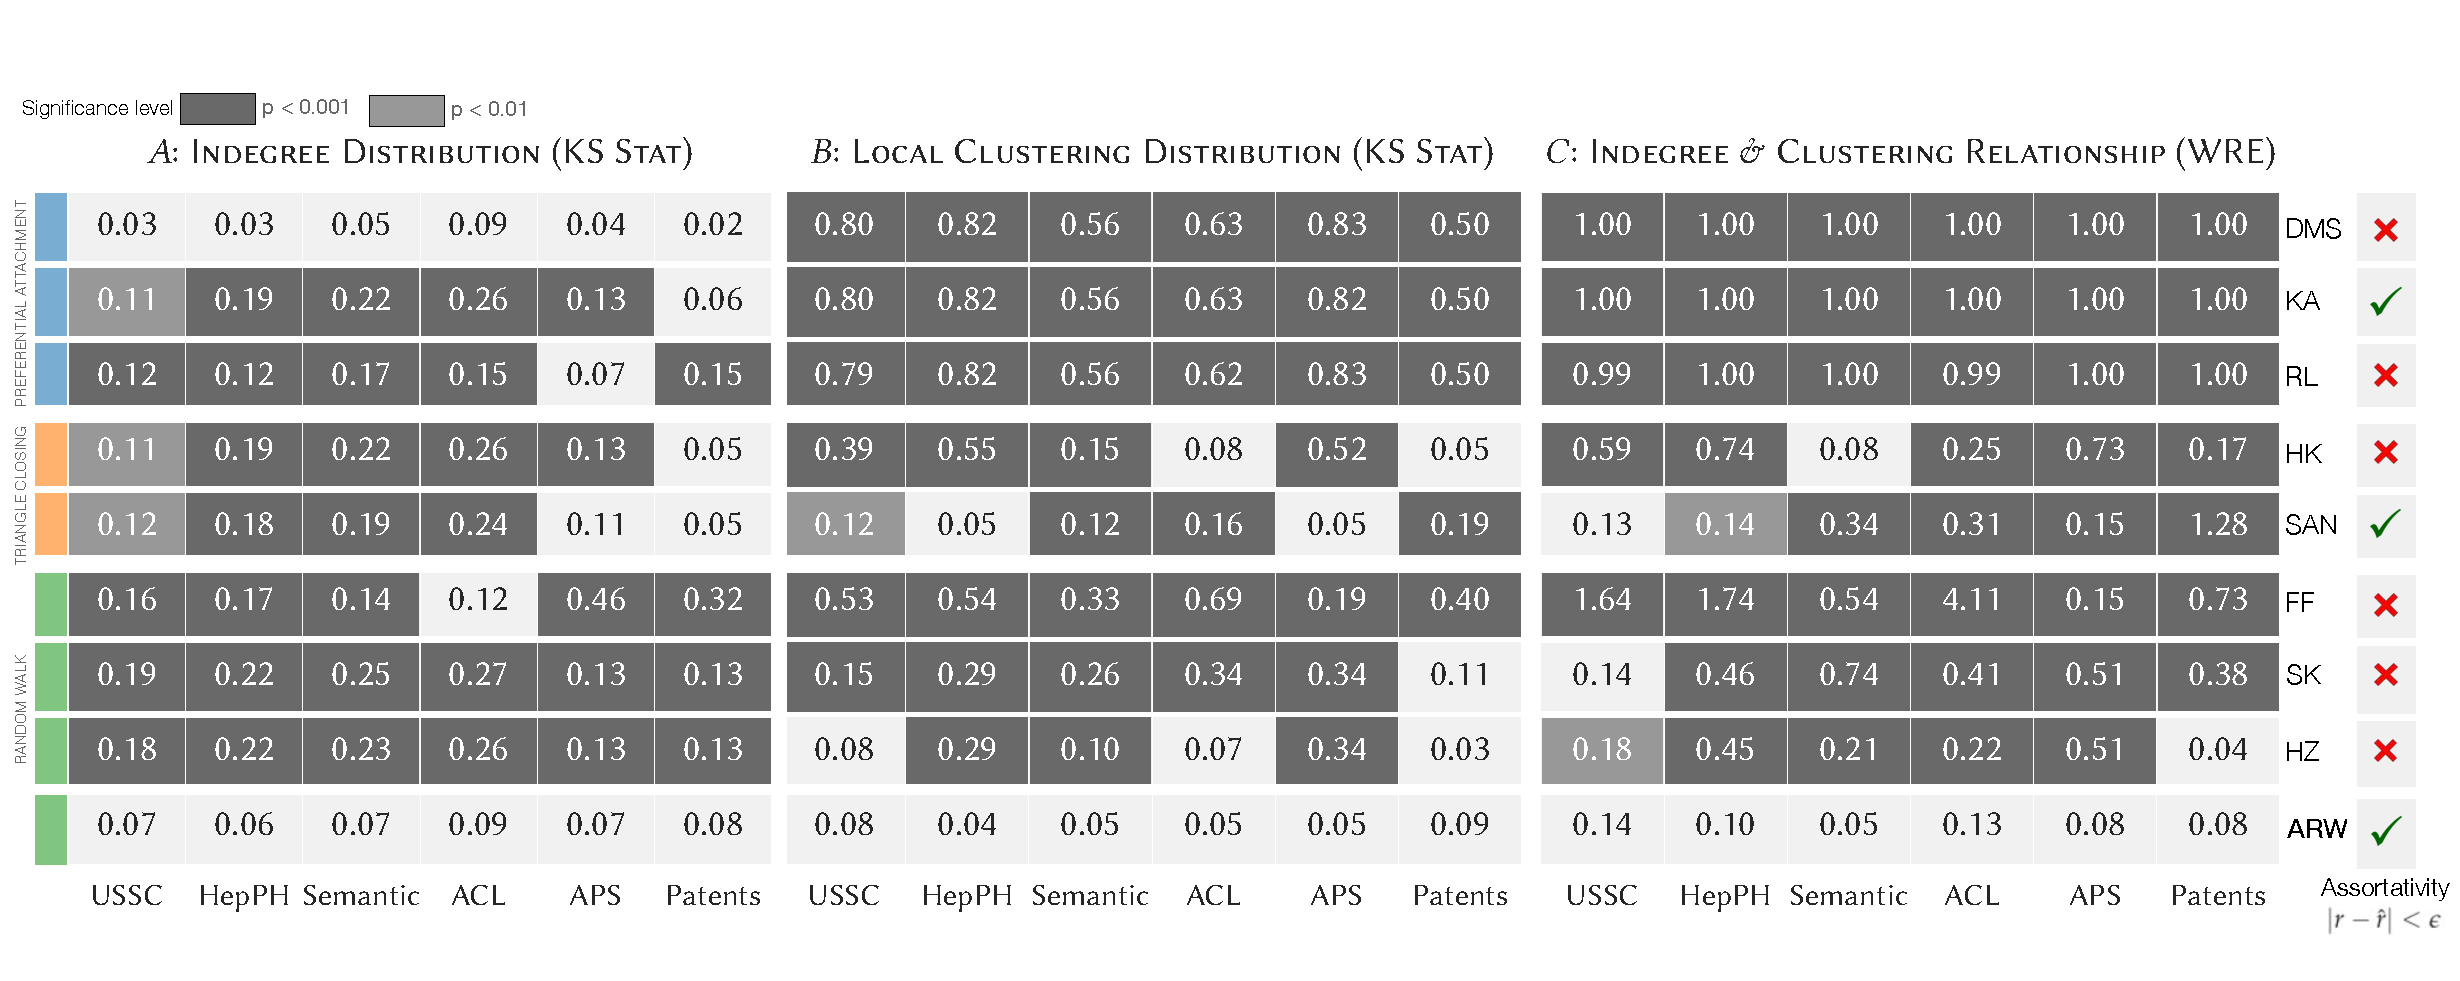
\includegraphics[width=.97\textwidth]{experiments}}
	\vspace{-16pt}
	\caption{
		Modeling network structure.
		% We assess the extent to which network models
		% fit key structural properties of six real-world networks.
		Tables 5A, 5B and 5C
		measure the accuracy of eight models in fitting key properties of real-world networks.
		% n-degree distribution,
		% local clustering distribution, in-degree \& clustering relationship
		% respectively and global attribute assortativity.
		% Existing models tend to underperform because they either disregard
		% the effect of factors such as triadic closure and/or homophily
		% or are unable to generate networks with varying structural properties.
		Our model, \texttt{ARW}, jointly preserves all four properties accurately and often
		performs considerably better than existing models:
		the cells are shaded gray or dark gray if the proposed model \texttt{ARW} performs
		better at significance level $\alpha=0.01$ ( \lightgraybg{ }) or $\alpha=0.001$ ( \darkgraybg{ })
		respectively.
	}
	\vspace{-10pt}
	\label{fig:exp_table}
\end{figure*}

\section{Modeling Network Structure}
\label{sec:Experiments}
In this section, we evaluate \texttt{ARW}'s efficacy in preserving
observed network structure relative to well-known growth models.
% In~\Cref{sub:Experimental Setup}, we begin by describing existing growth models and the evaluation metrics
% used in the experiments. Then, we discuss our results.

\subsection{Setup}
\label{sub:Experimental Setup}

% We first briefly summarize the existing models used in the experiments.
In this subsection, we introduce eight representative growth models
and describe evaluation metrics used to fit models to the datasets.

\textit{State-of-the-art Growth Models}. We compare \texttt{ARW} to eight
models representative of the key edge formation
mechanisms: preferential attachment, fitness, triangle closing and random walks.
Two of the eight models account for attribute homophily and preserve attribute mixing patterns,
as listed in~\Cref{table:models}.
% as listed below:
%
% 		\noindent{\textbf{(1) Dorogovtsev-Mendes-Samukhin model}} \cite{dorogovtsev2000structure}  (\texttt{DMS})
% 		is a preferential attachment model that generates directed scale-free graphs. In this model,
% 		the probability of linking to a node is proportional to the sum of its in-degree and ``initial attractiveness.''
%
% 		\noindent{\textbf{(2) Relay Linking model}} \cite{singh2017relay} (\texttt{RL}) comprises
% 		preferential attachment models for directed networks that use relay linking to model
% 		node popularity over time. We use the iterated preferential relay-cite (IPRC) variant, which best fits
% 		real-world network properties.
%
% 		\noindent{\textbf{(3) Kim-Altmann model}} \cite{kim2017effect} (\texttt{KA}) is a fitness-based model that defines
% 		fitness as the product of degree and attribute similarity. It generates {attributed} networks
% 		with assortative mixing and power law degree distribution.
% 		To generate directed networks, we modify \texttt{KA} to form directed edges to nodes in proportion to their in-degree.
%
% 		\noindent{\textbf{(4) Holme-Kim model}} \cite{holme2002growing} (\texttt{HK}) is a preferential attachment model
% 		that generates scale-free, clustered, undirected networks using a triangle-closing mechanism.
% 		To generate directed networks, we modify \texttt{HK} to form directed edges to nodes in proportion to their in-degree
% 		and close triangles in their undirected 1-hop neighborhood.
%
%
% 		\noindent{\textbf{(5) Social Attribute Network model}} \cite{gong2012evolution} (\texttt{SAN}) generates
% 		scale-free, clustered, attributed networks via attribute-augmented
% 		preferential attachment and triangle closing processes.
% 		We modify \texttt{SAN} to create directed edges and thereby produce directed networks.
% 		% We also note that
% 		% the edge formation mechanism in \texttt{SAN} considerably simplifies for bibliographic network datasets,
% 		% wherein all edges are formed at once.
%
% 		\noindent{\textbf{(6) Herera-Zufiria model}} \cite{saramaki2004scale} (\texttt{SK})
% 		is a random walk model that generates scale-free, undirected networks with tunable average clustering.
% 		In order to generate directed networks, we allow the random walk mechanism in \texttt{SK} to traverse edges in any direction.
%
% 		\noindent{\textbf{(7) Saramaki-Kaski}} \cite{herrera2011generating} (\texttt{HZ}) is a random walk model
% 		that generates scale-free networks with tunable average local clustering. To generate directed networks,
% 		we modify \texttt{HZ} to allow its random walk mechanism to traverse edges in any direction.
%
% 		\noindent{\textbf{(8) Forest Fire model}} \cite{leskovec2005graphs} (\texttt{FF}) is a recursive random walk model
% 		that can generate directed networks with shrinking diameter over time,
% 		heavy-tailed degree distributions and high clustering.

% \begin{enumerate}
% 	\item{\textbf{Dorogovtsev-Mendes-Samukhin model}} \cite{dorogovtsev2000structure}  (\texttt{DMS})
% 	is a preferential attachment model that generates directed scale-free graphs. In this model,
% 	the probability of linking to a node is proportional to the sum of its in-degree and ``initial attractiveness.''
%
% 	\item{\textbf{Relay Linking model}} \cite{singh2017relay} (\texttt{RL}) propose a set of
% 	preferential attachment models for directed networks, which use relay linking to explain the change in
% 	node popularity over time. We use the iterated preferential relay-cite (IPRC) variant, which best fits
% 	real-world network properties.
%
% 	\item{\textbf{Kim-Altmann model}} \cite{kim2017effect} (\texttt{KA}) is a fitness-based model that defines
% 	fitness as the product of degree and attribute similarity. It can generate \textit{attributed} networks
% 	with assortative mixing and heavy tailed degree distribution.
% 	To generate directed networks, we modify \texttt{KA} to form directed edges to nodes in proportion to their in-degree.
%
% 	\item{\textbf{Holme-Kim model}} \cite{holme2002growing} (\texttt{HK}) is a preferential attachment model
% 	that generates scale-free, clustered, undirected networks using an additional triangle-closing mechanism.
% 	We modify the model to create directed edges and thereby generate directed networks.
% 	To generate directed networks, we modify \texttt{HK} to form directed edges to nodes in proportion to their in-degree
% 	and close triangles in their undirected 1-hop neighborhood.
%
%
% 	\item{\textbf{Social Attribute Network model}} \cite{gong2012evolution} (\texttt{SAN}) generates
% 	scale-free, attributed networks with high clustering using attribute-augmented
% 	preferential attachment and triangle closing mechanisms.
% 	We modify the model to create directed edges and thereby generate directed networks. We also note that
% 	the edge formation mechanism in \texttt{SAN} considerably simplifies for bibliographic network datasets,
% 	wherein all edges are formed at once.
%
% 	\item{\textbf{Herera-Zufiria model}} \cite{saramaki2004scale} (\texttt{SK})
% 	is a random walk model that generates scale-free, undirected networks with tunable average clustering.
% 	In order to generate directed networks, we allow the random walk mechanism in \texttt{SK} to traverse edges in any direction.
%
% 	\item{\textbf{Saramaki-Kaski}} \cite{herrera2011generating} (\texttt{HZ}) is a random walk model
% 	that generates scale-free networks with tunable average local clustering. To generate directed networks,
% 	we modify \texttt{HZ} to allow its random walk mechanism to traverse edges in any direction.
%
% 	\item{\textbf{Forest Fire model}} \cite{leskovec2005graphs} (\texttt{FF}) is a recursive random walk model
% 	that can generate directed networks with properties such ash shrinking diameter over time,
% 	heavy-tailed degree distributions and high clustering.
% \end{enumerate}

% in~\Cref{table:models}.
\begin{table}[t]
 \center
 {
  \begin{tabular}[c]{llcc} \toprule
  Model &  Abbreviation & Type & Attributed? \\ \midrule
  Dorogovtsev et al.~\cite{dorogovtsev2000structure} & \texttt{DMS} & \texttt{PA} & \xmark  \\
  Relay Linking~\cite{singh2017relay} 						  & \texttt{RL} & \texttt{PA} & \xmark  \\
  Kim-Altmann~\cite{kim2017effect} 							  & \texttt{KA} & \texttt{PA} & \cmark  \\ \midrule
  Social Attribute Network~\cite{gong2012evolution} 	  & \texttt{SAN} & \texttt{PA+TC} & \cmark  \\
  Holme-Kim~\cite{holme2002growing} 						  & \texttt{HK} & \texttt{PA+TC} & \xmark  \\ \midrule
  Herera-Zufiria~\cite{herrera2011generating} 				  & \texttt{HZ} & \texttt{RW} & \xmark  \\
  Saramaki-Kaski~\cite{saramaki2004scale} 					  & \texttt{SK} & \texttt{RW} & \xmark  \\
  Forest Fire~\cite{leskovec2005graphs} 					  & \texttt{FF} & \texttt{RW} & \xmark  \\
   \bottomrule
  \end{tabular}
  \vspace{1mm}
  \caption{
  	  We evaluate the performance of our model \texttt{ARW} relative to 3 preferential attachment
	  (\texttt{PA}) models, 2 pref. attachment \& triangle closing (\texttt{PA+TC}) models and 3 random walk (\texttt{RW}) models.
  }
  \label{table:models}
 }
 \vspace{-10pt}
\end{table}

\textit{Ensuring Fair Comparison}. To ensure fair comparison, we modify existing models in three ways.
First, for \texttt{DMS}, \texttt{SAN}, \texttt{KA} do not have an explicitly defined initial graph,
so we use initialization method used for \texttt{ARW}, described in~\cref{sub:Model Fitting}. Second, we extend
models that use constant node outdegree $m$ by increasing outdegree over time $m(t)$
using the method described in~\cref{sub:Model Fitting}. In the absence of model-specific parameter estimation methods,
we use grid search to estimate the parameters of every network model, including \texttt{ARW},
using evaluation metrics and selection criterion described below.

\textit{Evaluation Metrics}.
We evaluate the model fit by comparing four properties of ${G}$ \& $\hat{G}$:
degree distribution, local clustering distribution, degree-clustering relationship
and attribute assortativity. We use Kolmogorov-Smirnov (\texttt{KS}) statistic to compare univariate
distributions and Weighted Relative Error (\texttt{WRE}) for the degree-clustering relationship.
\texttt{WRE} aggregates the relative error between the average local clustering $c(k)$ and $\hat{c}(k)$ of nodes with in-degree $k$ in $G$ and $\hat{G}$ weighted by the fraction of nodes with indegree $k$ in $G$.
% respectively; The relative error between $c(k)$ and $\hat{c}(k)$
% is weighted in proportion to the number of nodes with in-degree $k$ in $G$.

% \& local clustering distributions. We compare the degree-clustering relationship in $G$ and $\hat{G}$ using
% Weighted Relative Error (\texttt{WRE}), which aggregates the relative error
% between the average local clustering $c(k)$ and $\hat{c}(k)$ of nodes with in-degree $k$
% in $G$ and $\hat{G}$ respectively; The relative error between $c(k)$ and $\hat{c}(k)$
% is weighted in proportion to the number of nodes with in-degree $k$ in $G$.

Jointly preserving multiple structural properties is a multi-objective optimization
problem.
% model parameters that accurately preserve the degree distribution
% (i.e. low \texttt{KS} statistic) may not preserve the clustering distribution.
Therefore, for each model, the selection criterion for the grid search parameter estimation method
chooses the model parameters that minimizes the $\ell^2$-norm of the aforementioned evaluation metrics.
We normalize the metrics before computing the $\ell^2$-norm
to prevent unwanted bias towards any particular metric.
We note that the parameter sensitivity of the Forest Fire (\texttt{FF}) model necessitates
a manually guided grid search method.

% \begin{figure*}
% 	\centering
% 	\makebox[\textwidth][c]{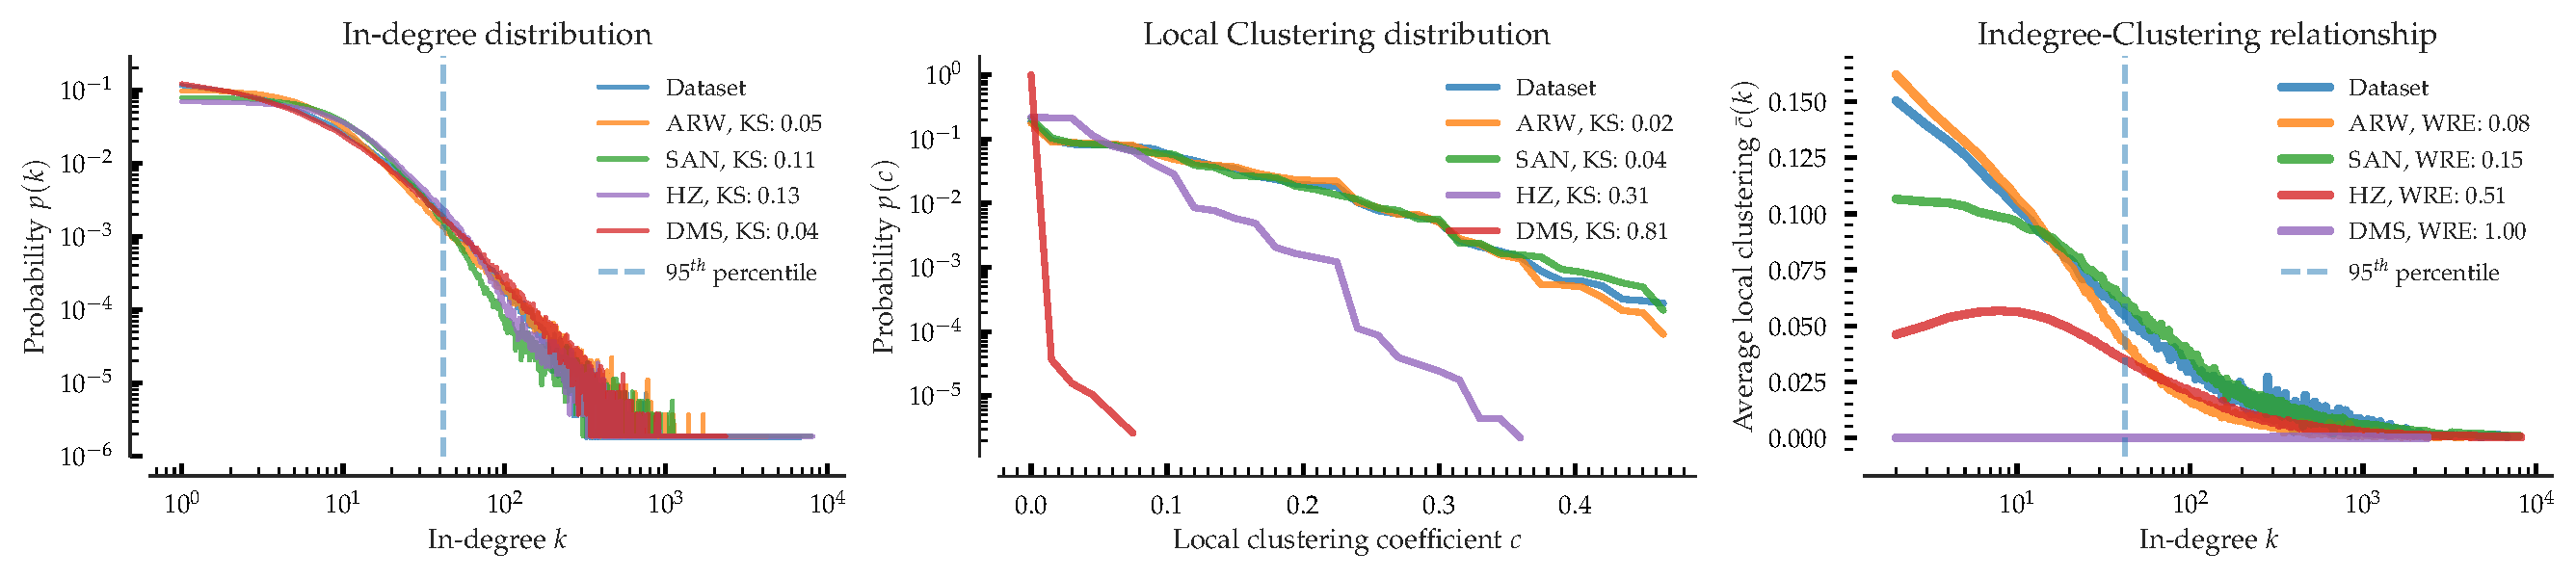
\includegraphics[width=\textwidth]{aps_fits}}
% 	\caption{
% 		Performance of \texttt{ARW} in accurately preserving key global structural properties
% 		of the \texttt{APS} network dataset relative to state-of-the-art, representative
% 		network models. Existing models such as \texttt{DMS} and \texttt{HK} cannot preserve high
% 		local clustering.
% 		% Although \texttt{SAN} preserves the univariate in-degree
% 		% and local clustering distributions, it does not account for the correlation between in-degree and clustering.
% 		Moreover, the triangle closing mechanism in \texttt{SAN} incurs high Weighted Relative Error (\texttt{WRE}) because
% 		it cannot explain why low in-degree nodes have high local clustering. \texttt{ARW} outperforms existing network models
% 		in jointly preserving all three structural properties, in addition to attribute mixing patterns.}
% 	\label{fig:aps_fits}
% \end{figure*}

% \vspace{-11pt}
\subsection{Results}
\label{sub:Experimental Results}

Now, we evaluate the performance of \texttt{ARW} relative to eight
models on the datasets introduced in~\Cref{sec:Datasets}.
For every pair of model and dataset, ~\Cref{fig:exp_table} tabulates the evaluation metrics
described in ~\Cref{sub:Experimental Setup}.
These metrics are averaged over 100 runs and measure the accuracy with which the fitted models
preserve key global network properties: degree distribution, local clustering distribution,
degree-clustering relationship and attribute assortativity.
% We do not compare the extent to which these models preserve attribute
% assortativity because the attribute related model parameters can be
% independently tuned up to arbitrary precision. Instead,

% To evaluate the performance of these models, we first fit each model
% to all network datasets $G$ in~\Cref{sec:Datasets}.
% Thereafter, we compare the structural properties of network dataset $G$ and network $\hat{G}$
% generated by the fitted model using evaluation metrics in~\Cref{sub:Experimental Setup}. We average out
% fluctuations in $\hat{G}$ over 100 runs.
 % data from these runs also help us conduct statistical tests.

We use one-sided permutation tests \cite{good2013permutation} to evaluate the relative
performance of \texttt{ARW}. If \texttt{ARW} performs better than a model on a dataset
with significance level $\alpha=0.01$ or $\alpha=0.001$, the corresponding cells in~\Cref{fig:exp_table}
are shaded gray ( \lightgraybg{ }) or dark gray (~\darkgraybg{ }) respectively.
We also group models that have similar edge formation mechanisms by color-coding the
corresponding rows in~\Cref{fig:exp_table}.  We use green ticks in~\Cref{fig:exp_table} to
annotate models that preserve attribute assortativity up to two decimal places.
% The performance of a model depends on the effectiveness of its underlying
% edge formation mechanisms. Therefore,  we group models (i.e. color-coded rows in table \ref{fig:exp_table}) based on their
% underlying edge formation mechanism: preferential attachment (blue), preferential attachment with
% triangle closing (orange) and random walk (green) mechanisms.

% ~\Cref{fig:exp_table} shows that existing models fail to jointly preserve
% {multiple} structural properties in an accurate manner. This is because existing
% models either disregard important mechanisms such as triadic closure and homophily
% or are not flexible enough to generate networks with varying structural properties.
% For instance, the preferential attachment model \texttt{DMS}
% can accurately fit the heavy-tailed degree distributions but does not
% account for local clustering.
% On the other hand, the attributed network model \texttt{SAN} tries to preserve
% all four properties but cannot do so accurately.

% \textbf{Preferential attachment models}: \texttt{DMS}, \texttt{RL}
% and \texttt{KA} preserve in-degree distributions but disregard
% clustering.
% \texttt{DMS} outperforms other models in accurately modeling
% degree distribution (\Cref{fig:exp_table}A) because its ``initial attractiveness''
% parameter can be tuned to adjust preference towards low degree nodes.
% Unlike \texttt{KA}, however, \texttt{DMS} cannot preserve global assortativity.
% \texttt{KA} outperforms \texttt{DMS} in preserving global assortativity because \texttt{KA}
% uses an attribute similarity parameter to model attribute mixing patterns.
% However, by assuming that successive edge formations are independent, both models disregard
% triadic closure and local clustering. (\Cref{fig:exp_table}B \&~\Cref{fig:exp_table}C).

% \textbf{Triangle Closing Models}: \texttt{HK} and \texttt{SAN} are preferential attachment models
% that use triangle closing mechanisms to generate scale-free networks with high average
% local clustering.
% Note that \texttt{HK} and \texttt{KA} fit degree distributions with the same \texttt{KS} statistic
% (\Cref{fig:exp_table}A) because they lack parameters that can generate varying degree distributions.
% While triangle closing leads to considerable improvement over \texttt{DMS}
% and \texttt{KA} in modeling local clustering, \texttt{HK} and \texttt{SAN} are not flexible enough
% to preserve local clustering in {all} datasets (see~\Cref{fig:exp_table}B \&~\Cref{fig:exp_table}C).
%  Nevertheless,
% barring one or two datasets in tables \ref{fig:exp_table}B and \ref{fig:exp_table}C,
% these models cannot accurately preserve the local clustering distribution and in-degree-clustering
% relationship observed in real networks.


We observe that existing models fail to \textit{jointly} preserve multiple properties
because they either do not account for mechanisms such as triadic closure and homophily
or are not flexible enough to generate networks with tunable structural properties.
Preferential attachment models---\texttt{DMS}, \texttt{RL}, \texttt{KA}---preserve in-degree
distributions (\Cref{fig:exp_table}A) but do not account for triadic closure. As a result, these models
do not preserve local clustering(\Cref{fig:exp_table}B \&~\Cref{fig:exp_table}C).
Models that use triangle closing mechanisms---\texttt{HK}, \texttt{SAN}---lead to considerable improvement
over \texttt{DMS} and \texttt{KA} in modeling local clustering. However, as shown in ~\Cref{fig:exp_table}B \&~\Cref{fig:exp_table}C, triangle closing is insufficient to preserve the skewed distribution over local
clustering in real-world networks with high accuracy.
Existing random walk models---\texttt{FF}, \texttt{SK}, \texttt{HZ}---
do not account for homophily and attribute mixing patterns.
\texttt{FF}, in particular, considerably overestimates local clustering because of its recursive edge
formation mechanism.
Conversely, \texttt{SK} and \texttt{HZ} are single-parameter network models that are not flexible
enough to generate networks with tunable structural properties. Please refer to the extended version of
our paper \footnote{\label{ft1} Extended version of the paper: https://arxiv.org/abs/1712.10195} for a detailed discussion of our results.

% \textbf{Existing random walk models}: \texttt{FF}, \texttt{SK}, and \texttt{HZ}
% cannot accurately preserve structural properties of real-world network datasets.
% The recursive approach in \texttt{FF} considerably overestimates local clustering.
% because nodes perform a probabilistic breadth-first search and link to \textit{all} visited/burned
% nodes.
% \texttt{SK} and \texttt{HZ} can control local clustering to some extent, as
% nodes perform a single random walk and link to each visited node with tunable probability $\mu$.
% However, both models lack control over the in-degree distribution. Furthermore, existing random walk models
% disregard attribute homophily and do not account for attribute mixing patterns.

\begin{figure}[b]
	\centering
	% \vspace{-3pt}
	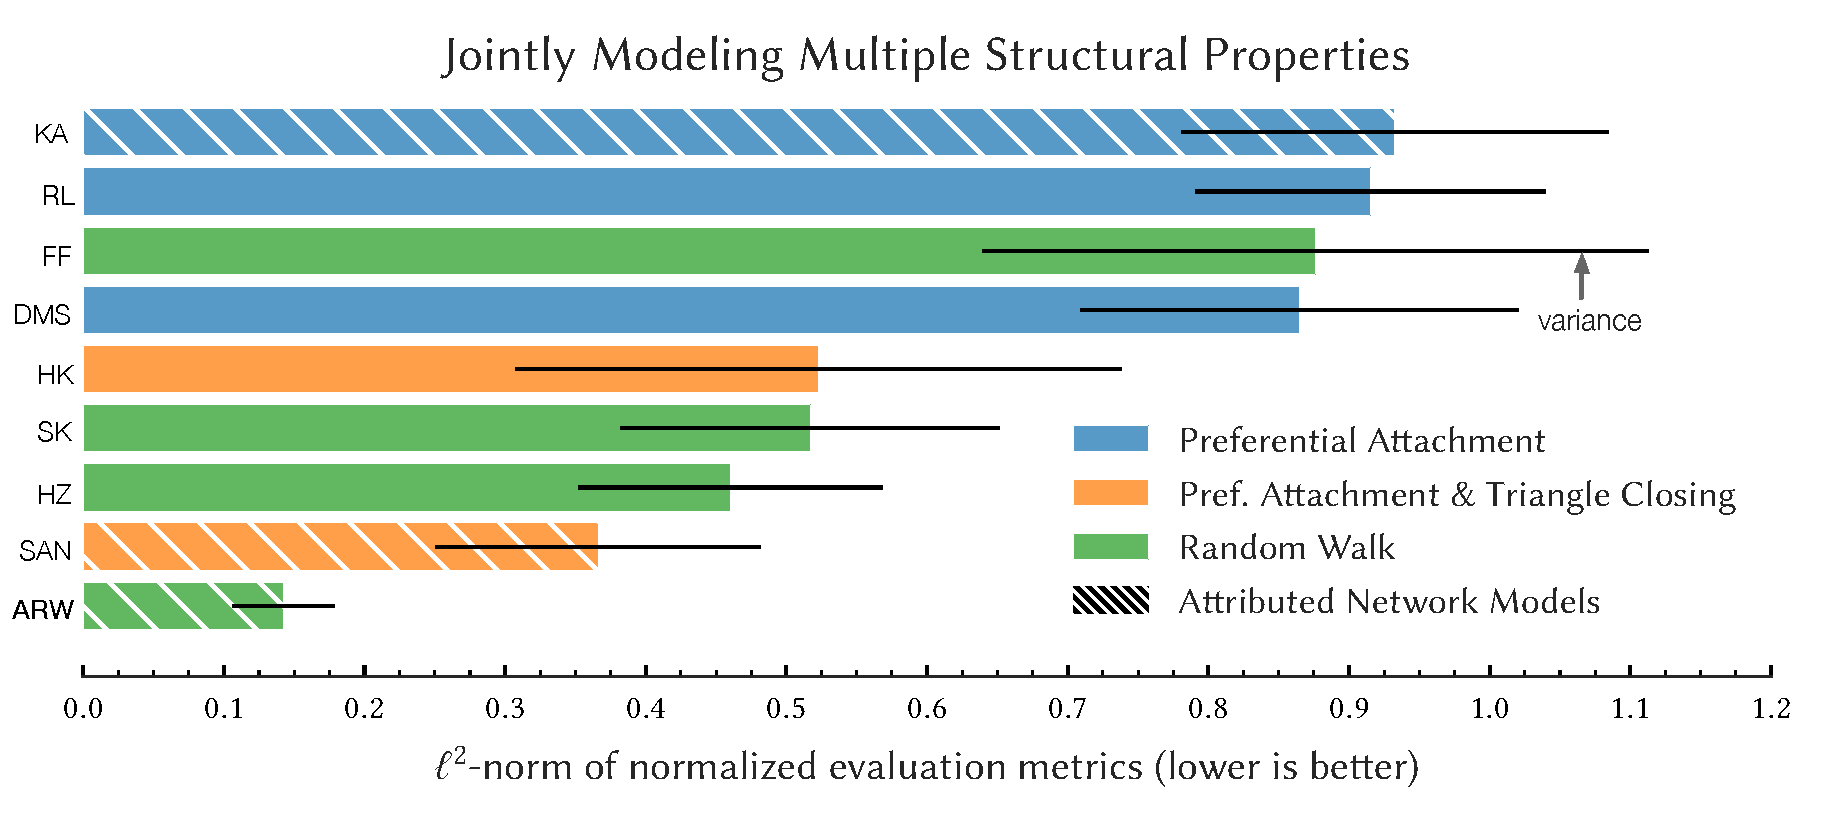
\includegraphics[width=.95\linewidth]{experiments_barplot}
	% \vspace{-10pt}
		\caption{\texttt{ARW} outperforms
			existing network models in jointly preserving key structural properties---in-degree
			distribution, local clustering distribution and degree-clustering relationship---
			by a significant margin of 2.5x-10x.
		}
		\label{fig:barplot}
\end{figure}

~\Cref{fig:exp_table} clearly indicates the effectiveness
of \texttt{ARW} in {jointly} preserving multiple
global network properties. \texttt{ARW} preserves observed
in-degree distributions by adjusting nodes' bias towards high degree nodes
using $\pout$.
% As a result, \texttt{ARW} accurately preserves
% in-degree distributions (\Cref{fig:exp_table}A), often significantly better
% than all models except \texttt{DMS}.
\texttt{ARW} matches the local clustering
distribution  (\Cref{fig:exp_table}B) and in-degree \& clustering relationship
(\Cref{fig:exp_table}C) with high accuracy using $\pjump$ and
$\plink$. \texttt{ARW} also preserves attribute assortativity using
the attribute parameters $\psame$ and $\pdiff$.

To summarize, \texttt{ARW} unifies multiple sociological phenomena into a single
mechanism using four parameters to jointly preserve key network properties significantly
better than existing models, as shown in~\Cref{fig:barplot},

% TODO: un-comment; commented out to fit paper to 10pages with author info
% In ~\Cref{fig:barplot}, we show that \texttt{ARW} improves upon the average $\ell^2$-norm
% of the second best performing model, \texttt{SAN}, by a significant margin of approximately 2.5x.
% Consider the \texttt{APS} dataset inn~\Cref{fig:aps_fits};
% we compare structural properties of the \texttt{APS} network to the properties of the networks
% generated by \texttt{ARW}, \texttt{SAN}, \texttt{HZ}, \texttt{DMS}; these models are collectively
% representative of key edge formation mechanisms and perform best among competing models that rely on
% similar mechanisms (e.g., preferential attachment). Clearly, \texttt{DMS} and \texttt{HK}
% cannot explain the high local clustering in the \texttt{APS} dataset.
% Conversely, \texttt{SAN} preserves local clustering distribution through its use of an attribute-augmented
% triangle closing mechanism. However, by coupling triangle-closing to preferential attachment, \texttt{SAN} does not account
% for the local clustering of the majority of nodes that have low in-degree.
% Unlike \texttt{ARW}, existing models cannot jointly preserve multiple structural properties in
% an accurate manner.


% \Cref{fig:barplot} illustrates the performance of network models in jointly
% modeling degree distribution, local clustering distribution and in-degree-clustering
% relationship. Preferential attachment models \texttt{KA}, \texttt{DMS} and
% \texttt{RL} perform poorly because they do not preserve clustering. \texttt{HK}
% and \texttt{SAN} perform better than \texttt{KA}, \texttt{DMS} and
% \texttt{RL} because of edge formation mechanisms that close triangles
% to preserve clustering and its relationship with degree to some extent. The proposed
% model \texttt{ARW} outperforms existing random walk models \texttt{HZ}, \texttt{SK}
% and \texttt{FF} by a considerable margin. Also,
% \texttt{ARW} significantly improves upon the average $\ell^2$-norm of the second best performing model,
% \texttt{SAN} by a margin of 2.5x


% key structural
% properties of real-world networks.




% \subsection{Parameter space of \textsc{RW} model}
%
% Through a series of extensive experiments, we observe that our model \textsc{RW} is able
% to model multiple structural characteristics of real-world networks. However, the fitted
% parameters are different for each dataset, suggesting possibly different
% local growth mechanisms in each network.~\Cref{table:rw_parameters}
% describes the best fitted parameters for five citation networks used in
% our experiments.
%
%
% \begin{table}[!h]
% \center
% \caption{ Best fittedparameters obtained after grid search for random walk model. }
% \label{table:rw_parameters}
% \resizebox{\columnwidth}{!}{%
% \begin{tabular}{@{}cccccc@{}}
%  & \multicolumn{1}{c}{\textit{USSC}} & \multicolumn{1}{c}{\textit{HEP-PH}}& \multicolumn{1}{c}{\textit{APS}}& \multicolumn{1}{c}{\textit{Patents}} & \multicolumn{1}{c}{\textit{Semantic}} \\ \toprule
%  $p_l$ & 0.80 & 0.80 & 0.15 & 0.25 & 0.40 \\
%  $p_j$ & 0.30 & 0.65 & 0.65 & 0.05 & 0.15 \\
%  $p_o$ & 0.95 & 0.95 & 0.80 & 1.00 & 0.95 \\
%  $p_r$ & 0.50 & 0.80 & 0.85 & 0.45 & 0.60 \\ \midrule
% \end{tabular}
% }
% \end{table}

% Weighted relative error (\texttt{WRE})
% is used to measure the similarity between the in-degree \& local clustering relationship in $G$ and $\hat{G}$:
% $$ \texttt{WRE}: \sum_{\text{Indeg.} k} P_{\textsc{g}}(k) \frac{c(k)-\hat{c}(k)}{c(k)} $$
% \texttt{WRE} is the weighted sum of the relative error between $c(k)$ and $\hat{c}(k)$,
% the average local clustering of nodes with degree $k$ in $G$ and $\hat{G}$ respectively;
% which aggregates the relative error between $c(k)$ and $\hat{c}(k)$,
% the average local clustering of nodes with degree $k$ in networks $G$
% and $\hat{G}$ respectively; The weight of each relative error term equals the probability
% mass $p_G(k)$ of in-degree $k$ in the observed network $G$.

%
% \begin{figure*}
%  \centering
%  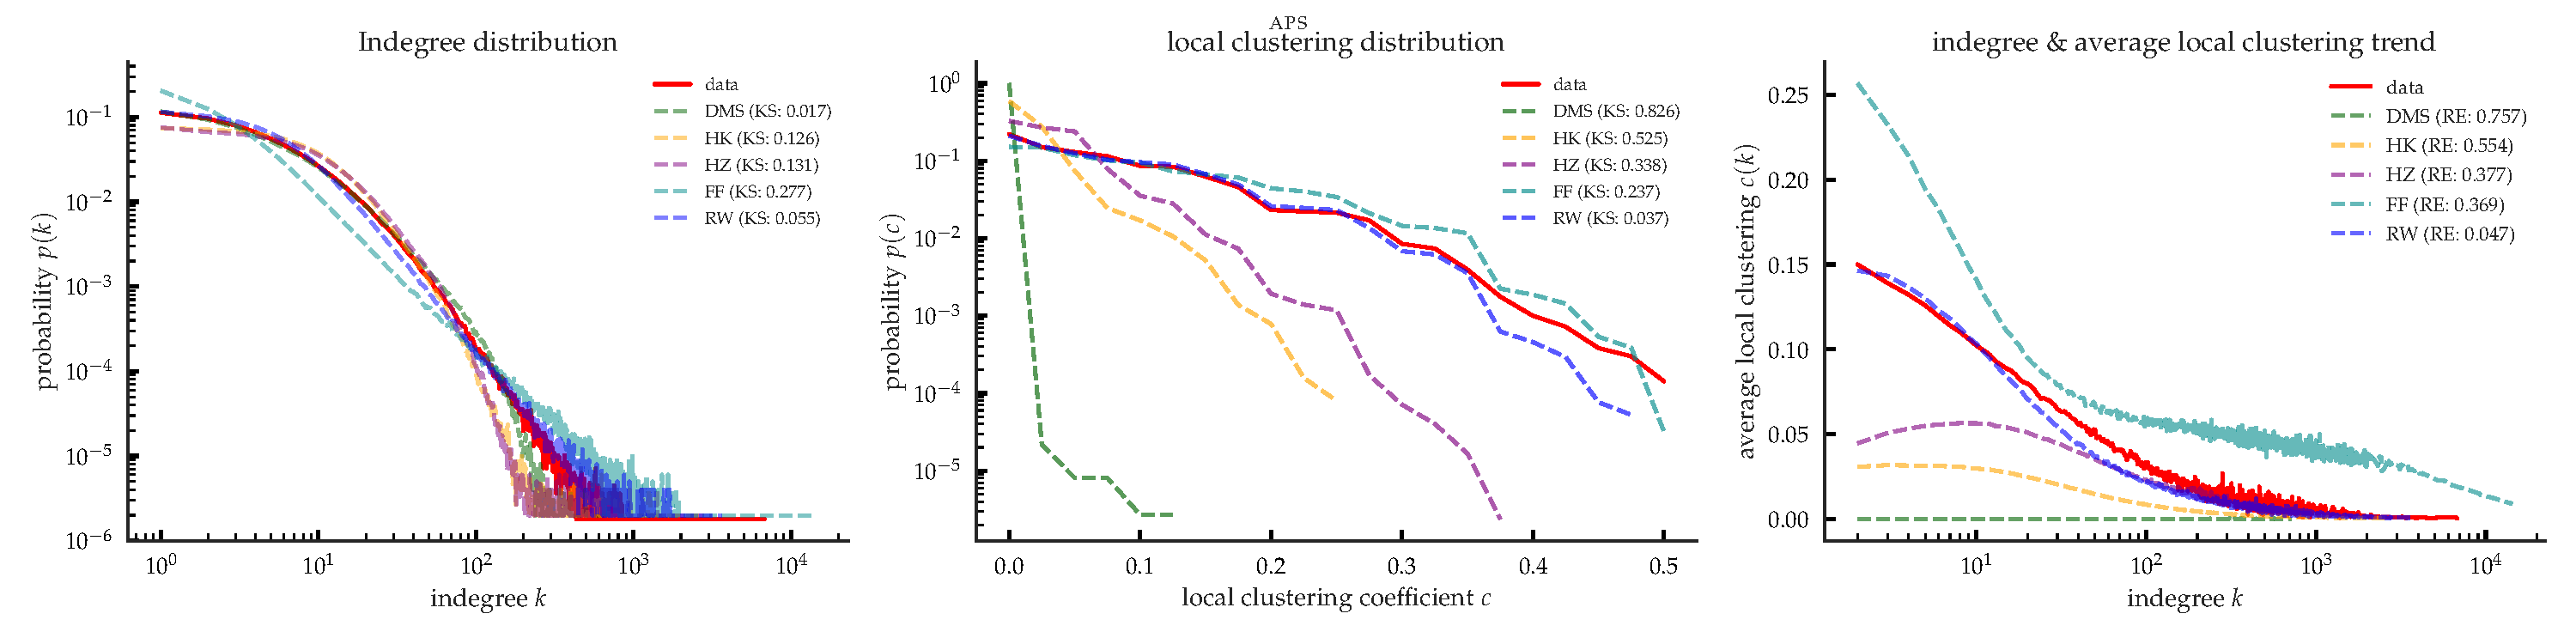
\includegraphics[width=\textwidth]{exp_aps}
%  \vspace{-12pt}
%
% \caption{Accuracy of growth models at preserving structural properties of \textsc{APS} network.
%  Our model \textsc{rw} outperforms the other in \textit{jointly} preserving heavy-tailed in-degree
%  distribution, skewed local clustering distribution and the in-degree \& average local clustering trend.}
%
% \label{fig:analysis}
% \end{figure*}


%
% \begin{enumerate}
% 	\item{\textbf{Dorogovtsev-Mendes-Samukhin model}} \cite{dorogovtsev2000structure}  (\texttt{DMS})
% 	is a preferential attachment model in which the probability of linking to a node is proportional
% 	to the sum of its in-degree and ``initial attractiveness.''
%
% 	\item{\textbf{Kim-Altmann model}} \cite{kim2017effect} (\texttt{KA}) is a fitness-based model that defines
% 	fitness as the product of degree and attribute similarity. It can generate \textit{attributed} networks with assortative mixing and
% 	heavy tailed degree distribution.
%
% 	\item{\textbf{Relay Linking model}} \cite{singh2017relay} (\texttt{RL}) propose a set of
% 	preferential attachment models that use relay linking to explain the change in node popularity over time.
% 	\footnote{We use the iterated preferential relay-cite (IPRC) variant, which best fits real-world network properties}
%
% 	\item{\textbf{Holme-Kim model}} \cite{holme2002growing} (\texttt{HK}) is a preferential attachment model
% 	which uses a triangle-closing mechanism to generate scale-free, clustered networks.
%
% 	\item{\textbf{Social Attribute Network model}} \cite{gong2012evolution} (\texttt{SAN}) generates
% 	scale-free, attributed networks with high clustering using attribute-augmented
% 	preferential attachment and triangle closing mechanisms.
%
% 	% We modify the model
% 	% to create directed edges and thereby generate directed networks.
%
% 	\item{\textbf{Herera-Zufiria model}} \cite{saramaki2004scale} (\texttt{SK})  is a random walk model
% 	that tunes the length of random walks to generate clustered networks with power law degree distributions.
%
% 	\item{\textbf{Saramaki-Kaski}} \cite{herrera2011generating} (\texttt{HZ}) is a random walk model
% 	that generates scale-free networks with tunable average local clustering.
%
% 	\item{\textbf{Forest Fire model}} \cite{leskovec2005graphs} (\texttt{FF}) is a recursive random walk model
% 	that preserves decreasing diameter over time, heavy-tailed degree distribution
% 	and high clustering.
% \end{enumerate}

% \clearpage
%!TEX root = ../draft.tex
\section{Modeling Local Mixing Patterns}
\label{subsec:LocalMixing}

The global assortativity coefficient quantifies
the average propensity of links to occur between similar nodes.
However, global assortativity is not a representative summary statistic of
heterogeneous mixing patterns observed in large-scale networks~\cite{peel2018multiscale}.
Furthermore, it does not quantify anomalous mixing patterns and fails to measure how mixing varies across a network.

We use local assortativity~\cite{peel2018multiscale} to measure varying
mixing patterns in an attributed network $G=(V,E,B)$ with attribute values $B=\{b_1...b_l\}$.
Unlike global assortativity that counts all edges between similar nodes, local assortativity
of node $i$, $r_l(i)$, captures mixing pattern in the local neighborhood of node
$i$ by using a locality biased weight distribution $w_i$. The distribution
$w_i$ reweighs edges between similar nodes based on how local they are to
node $i$.
As~\citet{peel2018multiscale} indicate, there are multiple ways
to define node $i$'s weight distribution $w_i$ other than the prescribed
personalized pagerank weight distribution, which is prohibitively expensive to compute
for all nodes in large graphs.
We define $w_i$ as a uniform distribution over $N_1(i)$, the set of nodes that
are at most 1 hop away from node $i$ to allow for a highly efficient
local assortativity calculation.
% EQUATION START
More formally, the local assortativity coefficient $r_l(i)$ of node $i$, with outdegree $m(i)$ and
attribute value $b(i)$ is defined as follows:
\begin{align*}
	\scriptsize r_l(i) = \frac{\overbrace{\frac{1}{|N(i)|}\sum\limits_{j \in N(i)}^{m(j) > 0} \sum_{k \in V} \frac{\mathcal{I}\{(j,k) \in E \wedge b(j)=b(k)\}}{m(i)} }^{\texttt{observed}}-\overbrace{\sum_{b \in B} e_{b}\cdot e_{b}}^{\texttt{random}}}{\underbrace{1}_{\max(\texttt{observed})}-\underbrace{\sum_{b \in B} e_{b} \cdot e_{b}}_\texttt{random}}
\end{align*}
Intuitively, $r_l(i)$ compares the observed fraction of edges between similar nodes
in the local neighborhood of node $i$ (\texttt{observed}) to the expected fraction
if the edges are randomly rewired (\texttt{random}).
% EQUATION END

As shown in~\Cref{fig:local_atty}, local assortativity distributions
of \texttt{ACL}, \texttt{APS} and \texttt{Patents} reveal anomalous, skewed
and heterophilic local mixing patterns that are not inferred via global assortativity.
\begin{figure}[h]
	\centering
	\vspace{-9pt}
	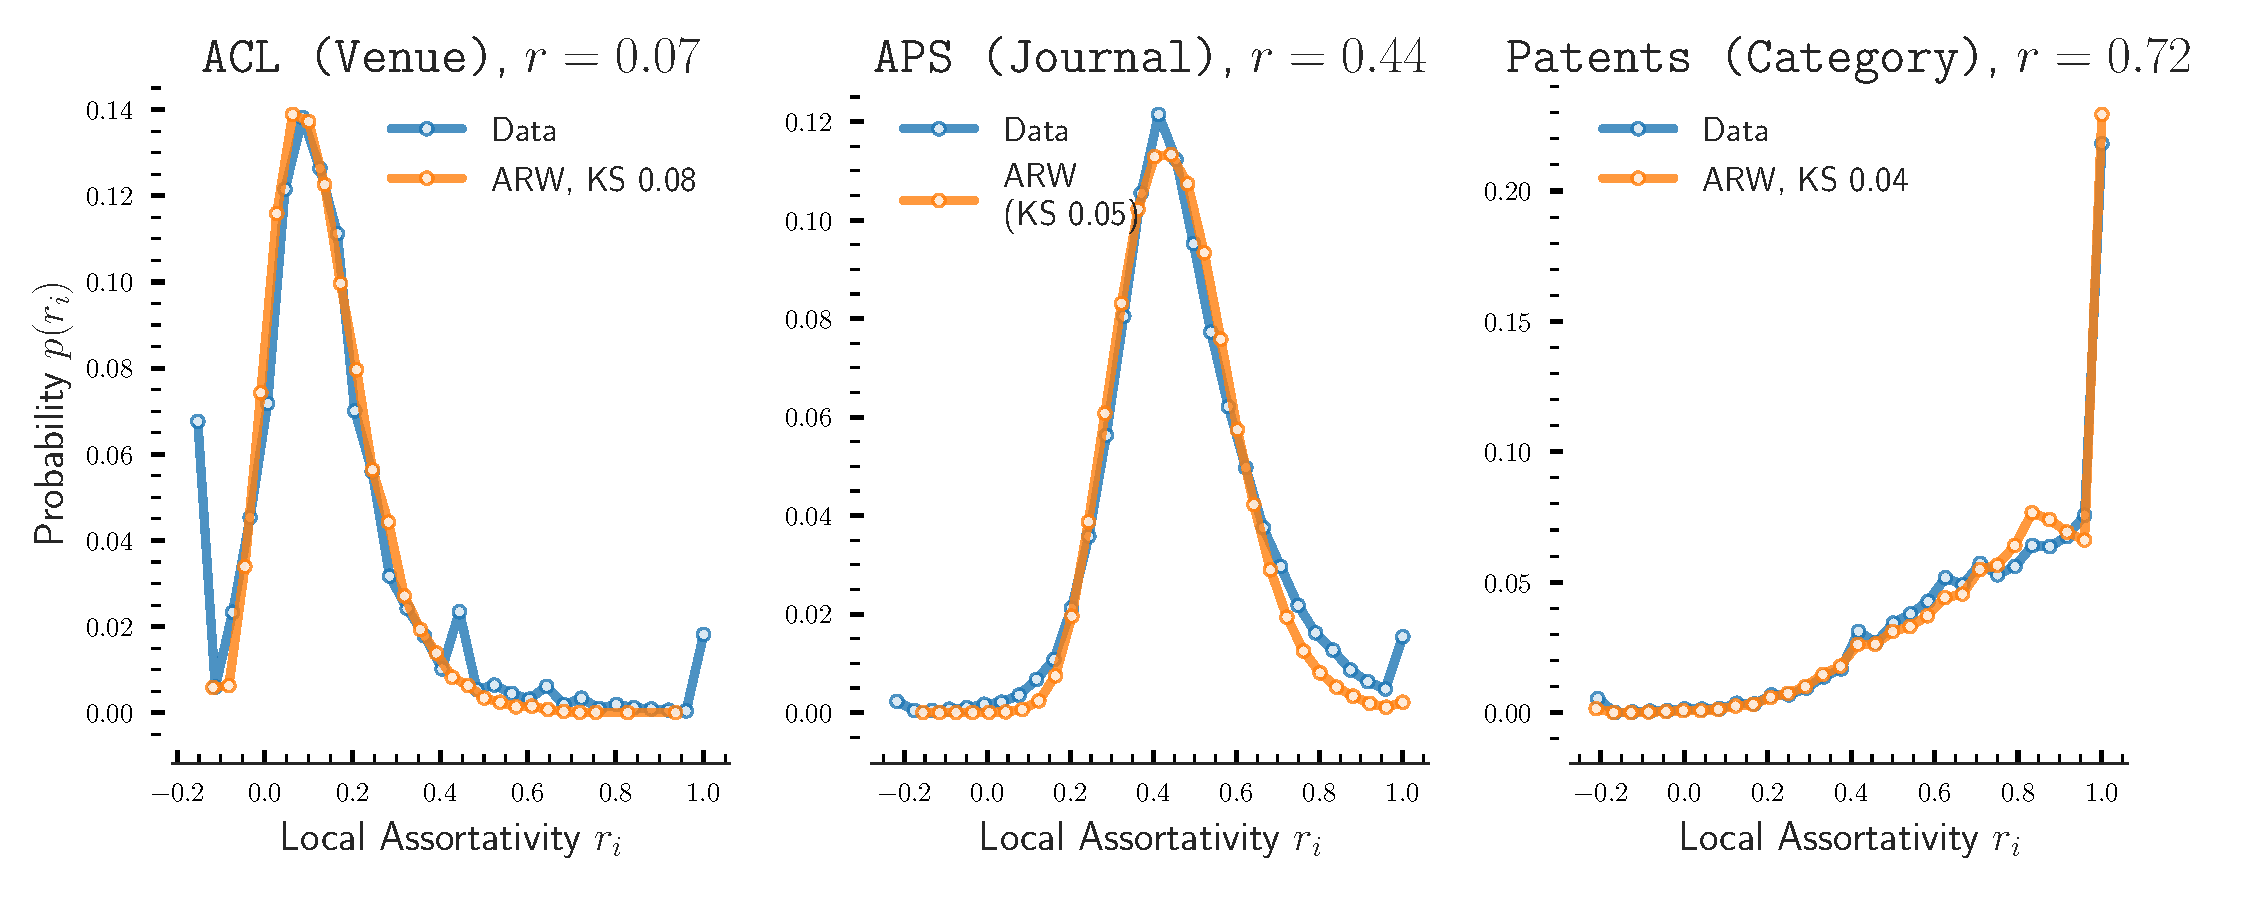
\includegraphics[width=\linewidth]{local_mixing}
	\caption{Local assortativity distributions of attributed networks \texttt{ACL}, \texttt{APS}
		and \texttt{Patents} reveal anomalous, skewed and heterophilic local mixing patterns.
		\texttt{ARW} accurately preserves local assortativity, but does not account for anomalous mixing patterns.}
	\label{fig:local_atty}
	\vspace{-8pt}
\end{figure}
Our model \texttt{ARW} can preserve
diverse local assortativity distributions with high accuracy even though nodes
share the same attribute parameters $\psame$ and $\pdiff$. This is because, in addition
to sampling attributes conditioned on time, \texttt{ARW}
incorporates multiple sources of stochasticity through its edge formation
mechanism. As a result, incoming nodes with fixed homophilic preferences can position
themselves in neighborhoods with variable local assortativity by (a) selecting a seed node in a region
with too few (or too many) similar nodes or (b) exhausting all its links before
visiting similar (or dissimilar) nodes.
We note that \texttt{ARW} is not expressive enough to model anomalous
mixing patterns; richer mechanisms such as sampling $\psame$ or $\pdiff$
from a mixture of Bernoullis are necessary to account for anomalous mixing patterns.

% \clearpage
%!TEX root = draft.tex

\section{Discussion}
\label{sec:Discussion}
In this section, we discussed the weaknesses of triangle closing mechanisms
(they considerably underestimate local clustering) and limitations of our model
\texttt{ARW}, including potential fixes.

% In this section, we discuss the weaknesses of the well-known triangle closing mechanism
% and the limitations of our model \texttt{ARW}.

\subsection{Dissecting the Triangle Closing Mechanism}
\label{ss:tc}

A set of network models (e.g., \texttt{SAN} \cite{gong2012evolution} \& \texttt{HK} \cite{holme2002growing})
use triangle closing mechanisms to generate networks with
varying average local clustering. However, our experimental results
in~\Cref{sub:Experimental Results} show that models that rely on triangle closing
cannot model the local clustering distribution or bivariate degree-clustering
relationship accurately. To understand why, we examine the degree-clustering
relationship in the \texttt{APS} network, in~\Cref{fig:triangle_closing}.
\begin{figure}[h]
    \centering
    \vspace{-7pt}
    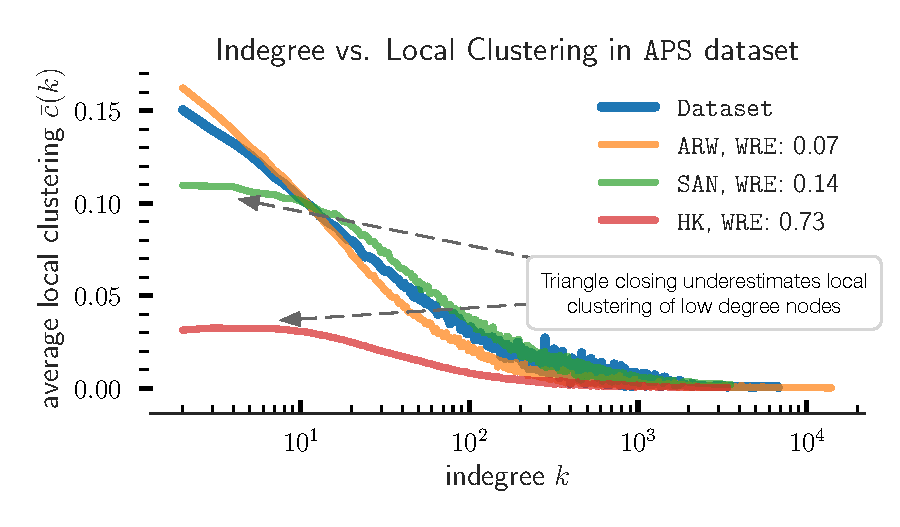
\includegraphics[width=.9\linewidth]{deg_cc_tc_om2f}
    \caption{Triangle closing mechanisms used in \texttt{SAN} \texttt{HK} fail to
    model average local clustering of low in-degree nodes. In contrast,
    to accurately preserve local clustering, \texttt{ARW} uses {random walks} to visit
    low in-degree nodes and ``closes triangles'' in their neighborhoods .}
    \label{fig:triangle_closing}
    \vspace{-5pt}
\end{figure}

\Cref{fig:triangle_closing} reveals that models based on triangle closing mechanisms,
\texttt{SAN} and \texttt{HK}, considerably underestimate the local clustering of
nodes that have low in-degree. This is because incoming nodes in \texttt{SAN} and \texttt{HK}
tend to close triangles in the neighborhood of high in-degree nodes to which they
connect via preferential attachment. Local clustering plateaus as in-degree decreases because
triangle closing along with preferential attachment fail to form connections in neighborhoods
of low in-degree nodes. In contrast, \texttt{ARW} accurately models the degree-clustering relationship
because incoming nodes initiate random walks in neighborhoods of seeds nodes that tend to have
low in-degree.

% \subsection{Measurement of Global Network Properties}
% Despite their widespread usage, summary statistics of global
% network properties such as global assortativity and average clustering have limited representative
% power. Unlike point estimates, distributional properties reveal variance, skewness and anomalies
% in network data.
% Notably, understanding local processes via distributional network properties
% guided the development of \texttt{ARW}, which consists of entirely \textit{local} processes
% that do not rely on global information (e.g. fitness values of all nodes).
% For instance, the \textit{skewed} clustering distribution and the relationship between clustering and
% degree necessitated the jump parameter $p_j$ in our model. The structural constraints imposed by the jump
% parameter amplify the effect of triadic closure and preserve high clustering
% observed in neighborhoods of low degree nodes.
% % Similarly, the variance in the
% % local assortativity distribution of real-world networks necessitated additional
% % stochasticity in the edge formation mechanism. As shown in
% % \cref{subsec:LocalMixing}, \texttt{ARW} accurately models varying local mixing
% % patterns because we augment seed selection to pick similar/dissimilar nodes
% % probabilistically. As a result, incoming nodes with fixed preferences can
% % initiate random walks in neighborhoods with varying local content properties.
% To summarize, we believe that the analysis and evaluation of \textit{distributional}
% network properties is crucial to accurately model network structure.

\subsection{\texttt{ARW} Limitations}
We discuss two limitations of our model \texttt{ARW}. First, \texttt{ARW} does not preserve the average
path length distribution of real-world networks. This is because the random walk
mechanism is inherently local and does not form {long-range connections} to bridge
distant regions of the network. Preliminary experiments on forming ``structural bridges''
by initiating multiple random walks for every node indicate a tradeoff
between modeling small average path length and high local clustering. Second,
we only consider citation network datasets where nodes form all edges at the time of joining.
This allows us to carefully analyze edge formation in the absence of confounding edge processes
such as edge deletion and edge creation between existing nodes. We can extend \texttt{ARW} to handle social networks, where individuals can form edges at any time. One way is to incorporate random walks that pause and resume intermittently, thus allowing for older nodes to connect with more recent arrivals.
% can jointly model edge formation processes between new and existing nodes in
% social networks;
Similarly, metapath based random walks can model interactions between
nodes of different types in heterogeneous information networks.












% In our future work, we plan to study the emergence of higher-order clustering
% \cite{yin2018higher} over time and the effect of homophily on the formation of
% temporal motifs \cite{paranjape2017motifs} via local processes such as \texttt{ARW}.

% and the importance of distributional network properties. Then, we briefly described
% simple methods to extend \texttt{ARW} and address current limitations of our model.
%
% extend our model to incorporate the effect of multiple
% nto \texttt{ARW}
% to explain the emergence of higher-order clustering \cite{yin2018higher} and study
% the effect of homophily on the formation of temporal motifs \cite{paranjape2017motifs}.
% We believe that local processes such as random walks

% In this work, we address the problem of modeling growth of real-world
% bibliographic networks. Our proposed model is an improvement over existing
% random walk growth models that preserves multiple key network structural
% properties such as degree distribution, clustering coefficient distribution and their
% joint relationship. A standard modeling assumption is that \textit{new} nodes joining a
% network can potentially make connection to \textit{any} existing node in the network in
% some prescribed manner. Our experiments suggest that local link formation
% process in which \textit{new} nodes explore local network neighborhoods
% and makes connections in the explored locality can explain multiple structural
% properties of real-world networks.
%
% We note that clustering coefficient is an important characteristic of
% real-world networks. We observe that clustering is not
% uniformly distributed over the network and clustering at nodal level to be
% highly right skewed. The skewness implies that some parts of the network is more
% clustered than the other parts. In addition to skewness, clustering at nodal
% level is correlated to nodal degree. We propose a random-walk model the that
% gives rise to prominent characteristics of the network such as skewed local
% clustering.
%
% Finally, we show, via attributed network modeling, the extensibility
% of our proposed random walk model. The modeling suggests that our
% growth model can be adapted to account for growth of other kinds of
% information such as attributes and link types. Modeling other informative
% networks such as multiplex networks and heterogeneous information networks
% should be the focus of future work.

% \section{Limitations}
% Now, we discuss the limitations of our work. First, our work is limited to
% bibliographic datasets because of availibility of temporal data. We use the
% temporal out-degree sequence of incoming nodes in the network to model the
% network growth. In absence of temporal information, our growth model can be
% adapted by relying on the densification power law exponent. Second, our random
% walk model is sensitive to the initial graph. Since random walks explore the
% locality of a network and cannot access the entire network , the initial graph
% should have a giant weakly connected component. We recognise that the
% intialization problem can be addressed by having non-local source of information
% such as multiple seed nodes. Third, we note that our model fails to preserve
% certain network properties such as path length distribution. This is because
% our model does not account for nodes that serve as ``local bridges'' in the network.
% Modeling local and global processes simulatenously in a joint random walk model
% should lead to preservation of the discussed key network properties.

% \clearpage
%!TEX root = draft.tex
\section{Related Work}
\label{sec:Related Work}
network growth models seek to explain a subset of structural properties observed in real
networks. Well-known network growth models can be broadly categorized by their
edge formation mechanism(s):

% PA
\textbf{Preferential Attachment \& Fitness}
In preferential attachment and fitness-based models \cite{bell2017network,medo2011temporal,bianconi2001bose,caldarelli2002scale}, a new node $u$ links to an existing node $v$
with probability proportional to the attachment function $f(k_v)$, a function of
either degree $k_v$ or fitness $\phi_v$ of node $v$; Node fitness is defined as a dimensionless
measure of node attractiveness.
For instance, linear preferential attachment functions
\cite{barabasi1999emergence,kumar2000stochastic,dorogovtsev2000structure} lead to
power law degree distributions and small diameter \cite{bollobas2004diameter}
and attachment functions of degree \& node age \cite{wang2013quantifying}
can preserve realistic temporal dynamics.
Extensions of preferential
attachment \cite{mossa2002truncation,zeng2005construction,wang2009local} that
incorporate resource constraints
disregard network properties other than power law degree distribution and small diameter.
Additional mechanisms are necessary to explain network properties
such as clustering and attribute mixing patterns.

% The structural
% properties these models preserve depends on the exact definition of
% the attachment function $f$.
% The attachment function $f$ that controls edge formation in preferential
% attachment models directly impacts degree distribution
% whereas
% sublinear attachment functions \cite{krapivsky2000connectivity,dereich2013random} can generate
% networks with stretched exponential degree distribution.
% In~\Cref{sec:Experiments}, we observe that \texttt{DMS}, a preferential attachment model with
% an affine attachment function, can accurately fit the degree
% distribution of real-world networks.
% Both mechanisms disregard triadic closure and
% resource constraints.

% fitness
% In fitness growth models
% \cite{bell2017network,medo2011temporal,bianconi2001bose,caldarelli2002scale},
% the rate at which an existing node $u$ acquires links is proportional to its
% fitness $\phi_u$, a dimensionless measure of node attractiveness based on
% intrinsic nodal properties that influence edge formation. The structural
% properties a fitness-based model preserves depends on the exact definition of
% fitness.
% For example, models that define fitness as a function of degree and
% node recency \cite{wang2013quantifying} or attribute similarity
% \cite{de2013scale} can preserve realistic temporal dynamics such as popularity
% decay and assortative attribute mixing patterns.
% Since new nodes form
% each edge \textit{independently}, fitness-based models such as \texttt{HPA} do
% not incorporate triadic closure and resource constraints.
% %  Additional mechanisms %
% are necessary to preserve the high local clustering or the degree-clustering %
% correlation observed in real networks.

\textbf{Triangle Closing}
A set of models
\cite{holme2002growing,klemm2002highly,leskovec2008microscopic}
incorporate triadic closure using triangle closing mechanisms,
which increase \textit{average} local clustering by forming edges between nodes
with one or more common neighbors. However, as explained in \cref{ss:tc}, models
based on preferential attachment and triangle closing do not preserve the local
clustering of low degree nodes.

\textbf{Attributed network models}
Attribute network growth models \cite{de2013scale,karimi2017visibility,gong2012evolution,zheleva2009co}
account for the effect of attribute homophily on edge formation and preserve mixing patterns.
Existing models can be broadly categorized as (a) fitness-based model that define fitness as a function of
attribute similarity and (b) microscopic models of network evolution that require
complete temporal information about edge arrivals \& deletion. Our experiment
results in \cref{sub:Experimental Results} show that well-known attributed network models
\texttt{SAN} and \texttt{KA} preserve assortative
mixing patterns, degree distribution to some extent, but not local clustering
and degree-clustering correlation.

\textbf{Random walk models}
% Random walk models, first introduced by Vazquez \cite{vazquez2000knowing,
% vazquez2003growing}, jointly explain the emergence of multiple properties
% observed in real networks under constraints of partial access and limited
% information.
first introduced by Vazquez \cite{vazquez2000knowing}, random walk models are inherently local.
Models \cite{blum2006random} in which
new nodes only link to terminal nodes of short random walks generate
networks with power law degree distributions \cite{chebolu2008pagerank} and
small diameter \cite{mehrabian2016sa} but do not preserve clustering. Models
such as \texttt{SK} \cite{saramaki2004scale}
and \texttt{HZ} \cite{herrera2011generating}, in which new nodes probabilistically link to
each visited nodes incorporate triadic closure but are not flexible enough to preserve
\textit{skewed} local clustering of real-world networks, as shown in \cref{sub:Experimental Results}.
We also observe that recursive random walk models such as \texttt{FF} \cite{leskovec2005graphs}
preserve temporal properties such as shrinking diameter but considerably overestimate local clustering
and degree-clustering relationship of real-world networks.
Furthermore, existing random walk models disregard the effect of homophily and do not model attribute mixing
patterns.

\textbf{Recent Work}
P{\'a}lovics et al. \cite{palovics2017raising} use preferential \& uniform
attachment to model the decreasing power law exponent of real-world, undirected
networks in which average degree increases over time. Singh et al.
\cite{singh2017relay} (\texttt{RL}) augment preferential attachment to explain
the shift in popularity of nodes over time via the concept of relay linking.
Both models do not incorporate mechanisms to preserve clustering, attribute
mixing patterns and resource constraints that affect how individuals form edges
in real-world networks.

To summarize, existing models do not explain how resource constrained and local processes
\textit{jointly} preserve multiple global network properties of attributed networks.
To the best of our knowledge, \texttt{ARW} is the first model that unifies multiple
sociological phenomena into an entirely local process to model
network structure \textit{and} attribute mixing patterns.
We point the reader to
extensive surveys \cite{newman2003structure,albert2002statistical} of network growth models
for more information.

% Growth models that account for the effect of attribute homophily on edge formation
% jointly preserve assortative mixing patterns and a few structural properties observed
% in real-world attributed networks. These models
% can be broadly categorized as (a) fitness-based model that define fitness as a
% function of attribute similarity and (b) microscopic models of network
% evolution that require complete temporal information about edge arrivals \&
% deletion. In~\Cref{sub:Experimental Results}, we observe that fitness-based
% models \cite{de2013scale,karimi2017visibility} such as \texttt{HPA} and
% microscopic models \cite{gong2012evolution,zheleva2009co} such as \texttt{SAN}
% can preserve assortative mixing patterns and degree distribution to some extent,
% but disregard clustering, degree-clustering correlation and resource
% constraints.


% Preferential attachment and fitness-based mechanisms make two strong assumptions.
% First, both mechanisms require nodes to link
% uniformly at random to \textit{any} node in the network \textit{or} have explicit
% knowledge of the degree/fitness of every node in the network.
% This assumption is
% unrealistic because individuals in real networks form edges under partial
% information and limited access constraints.
% Second, by assuming that successive edge formations are independent,
% both mechanisms
% disregard the effect of triadic closure on edge formation.
% Extensions of preferential
% attachment \cite{mossa2002truncation,zeng2005construction,wang2009local} that
% incorporate resource constraints disregard network properties other than
% power law degree distribution and small diameter.
%  by restricting access to newly added nodes or a
% small set of nodes uniformly sampled from the network
% . However, these models are
% simple, proof-of-concept methods that disregard network properties other than
% power law degree distribution and small diameter.
% Another set of models
% \cite{holme2002growing,klemm2002highly,leskovec2008microscopic}, including \texttt{HK},
% incorporate triadic closure using triangle closing mechanisms, which increase \textit{average} local
% clustering by forming edges between nodes with one or more common neighbors.
% However, as shown in~\Cref{sec:Experiments}, \texttt{HK} cannot preserve
% the \textit{skewed} clustering distribution and degree-clustering correlation
% observed in real networks.
% and contradict a key empirical finding: the
% probability of edge formation increases as a function of neighborhood overlap
% \cite{kossinets2006empirical}.


% Random walk models, first introduced by Vazquez \cite{vazquez2000knowing,
% vazquez2003growing}, jointly explain the emergence of multiple properties
% observed in real networks under constraints of partial access and limited
% information. Unlike previous mechanisms, random walk models are inherently local;
% New nodes initiate random walk(s) to explore neighborhoods of
% existing nodes and link to visited nodes. Models \cite{blum2006random} in which
% new nodes nodes only link to terminal nodes of short random walks generate
% networks with power law degree distributions \cite{chebolu2008pagerank} and
% small diameter \cite{mehrabian2016sa} but without high clustering. Models
% \cite{herrera2011generating,saramaki2004scale} such as \texttt{SK} \&
% \texttt{HZ}, in which new nodes initiate a single random walk and
% probabilistically link to visited nodes, implicitly incorporate triadic closure
% and can generate networks with high average local clustering. Moreover,
% recursive random walk models \cite{leskovec2005graphs,vazquez2003growing} such
% as \texttt{FF}, wherein nodes perform a probabilistic breadth first search to
% link to existing nodes, preserve temporal properties such as shrinking
% diameter. However, our experimental results in~\Cref{sec:Experiments} suggest
% that these models --- \texttt{HZ}, \texttt{SK} and \texttt{FF} --- do not accurately preserve
% the clustering distribution and/or degree-clustering correlation observed
% in real networks. Existing random walk models also disregard the effect of homophily on network formation.



% There has been extensive work on network growth models that \textit{explain} how
% a subset of structural properties of real world networks emerge from edge
% formation mechanisms over time. In this section, we describe four edge formation mechanisms underlying network
% growth models: preferential attachment \cite{jeong2003measuring} and its
% extensions, fitness \cite{albert2002statistical}, triangle closing mechanisms
% \cite{bianconi2014triadic} and random walks \cite{vazquez2000knowing}.  These
% edge formation mechanisms explain the emergence of multiple structural
% properties of real networks, but make one or more strong assumptions.

% Preferential attachment models such as the Barabasi-Albert model \cite{barabasi1999emergence} and Vertex
% Copying model \cite{kumar2000stochastic} explain the emergence of power law degree
% distributions of the form $p(k) = c\cdot k^{-\alpha}$, commonly observed in real
% networks. In preferential attachment models, new nodes that join the network
% form edges to existing nodes with probability proportional to their degree. This
% implies that high degree nodes accumulate edges quicker than low degree nodes.
% An intuitive explanation of preferential attachment is that new nodes are more
% likely to link to ``popular'' high degree nodes than relatively unknown, low
% degree nodes. However, preferential attachment implicitly assumes that edge
% formation depends only on degree and cannot explain why real networks exhibit
% high clustering or degree distributions that do follow power law.

% Unlike preferential attachment models, fitness models are flexible enough to
% generate networks with varying degree distributions and degree correlation. The
% inability of preferential attachment to preserve multiple structural properties
% suggests that factors other than degree influence edge formation. In fitness
% models, new nodes that join the network form edges to existing nodes with
% probability proportional to their fitness. The fitness $\phi_i $ of node $v_i$
% is a function of intrinsic nodal properties that influence edge formation. The
% structural properties a fitness model preserves depends on the exact definition
% of fitness. For example, the fitness model introduced in \cite{bianconi2001bose} increases fitness
% as a function of degree and node recency. This can preserve temporal dynamics
% such as decay in popularity \cite{wang2013quantifying} of old nodes in citation networks. Simpler fitness
% models can generate degree distributions that follow power law, exponential or
% lognormal \cite{medo2011temporal} distributions. However, since new nodes form each edge
% \textit{independently}, fitness alone cannot explain the emergence of high local
% clustering or the bivariate relationship between degree and clustering observed
% in real networks.

% Edge formation mechanisms proposed by the above network growth models make
% two strong assumptions.
% \begin{itemize}
%     \item \textbf{Complete access to information}
%     These mechanisms require nodes to link uniformly at random to \textit{any}
%     node in the network or have explicit knowledge of the degree/fitness of
%     every node in the network. This assumption is unrealistic because nodes in
%     real networks form edges partial information and limited access constraints.
%
%     \item \textbf{Successive edge formations are independent} There is a strong, implicit
%     assumption that a node's decision to link to another node is independent of the
%     nodes to which it has already linked. This assumption contradicts a key empirical
%     finding that the probability of edge formation increases as a function
%     of neighborhood overlap in social, information and citation networks.
% \end{itemize}
%
% % triangle closing
% Extensions of preferential attachment and fitness models \cite{holme2002growing,klemm2002highly} using triangle
% closing mechanisms explain why social \& information networks have high
% average local clustering \cite{newman2001clustering}. In these models, a new node that joins the network
% ``closes triangles'' by linking to neighbors of nodes it has already linked to
% based on degree or fitness. Closing triangles increases the number of edges
% between neighbors, thereby increasing the average local clustering. Triangle
% closing mechanisms essentially model triadic closure, a sociological process
% that explains why two nodes with mutual neighbor(s) have an increased
% probability of connection. In~\Cref{sec:Experiments}, we show that these
% models are not flexible enough to capture the skewness and variance in
% clustering distributions of real networks.
%
% % limited info
% A few models \cite{mossa2002truncation,zeng2005construction,wang2009local} adapt
% preferential attachment and fitness to model network growth under constraints of
% limited access and information. These models incorporate constraints by
% restricting access to recent nodes or a small set of nodes uniformly sampled
% from the network. However, these simple models are proof-of-concept methods that
% do not generate networks with varying degree distributions and realistic local
% clustering distributions.

% Random walk models jointly explain multiple structural properties of real
% networks under constraints of limited access and information. New nodes explore
% neighborhoods of existing nodes without any assumption of global information and
% use simple rules to form edges. New nodes that join the network perform one or
% more random walks to link to existing nodes. For example, the Random Surfer
% model \cite{blum2006random}, in which new nodes link to the terminal nodes of short random walks,
% generate networks that exhibit power law degree distributions. Importantly, this
% model explains preferential attachment as an \textit{emergent} property of local
% proceses. Random walk models in which new nodes perform random walk(s) and link
% to \text{any} visited node incorporate triadic closure and generate networks
% with heavy tailed degree distribution and high local clustering \cite{herrera2011generating}. In~\Cref{sec:Experiments}, we show that models based on random walks outpeform
% well-known \textit{global} edge formation mechanisms in preserving structural
% properties of citation networks. However, current random walk models are
% either inflexible or too simple to accurately capture local clustering observed
% in real networks.

% % summary
% To summarize, network growth models use global or local edge formation mechanism(s) to
% explain structural properties of real networks. Structural properties preserved
% by global edge formation mechanisms such as preferential attachment can be
% preserved by local processes such as random walks as well. However, unlike
% random walks, extensions of global processes such as preferential attachment \&
% fitness models make strong, unrealistic assumptions.
%!TEX root = ../main.tex
\vspace{-6pt}
\section{Conclusion}
\label{sec:Conclusion}
In this paper, we proposed a simple, interpretable model of attributed network
growth. \texttt{ARW} grows a directed network in the following manner: an
incoming node selects a seed node based on attribute similarity, initiates a
biased random walk to explore the network by navigating through neighborhoods of
existing nodes, and halts the random walk after connecting to a few visited
nodes. To the best of our knowledge, \texttt{ARW} is the first model that
unifies multiple sociological phenomena---bounded rationality; structural
constraints; triadic closure; attribute homophily; preferential
attachment---into a single local process to model global network structure
\textit{and} attribute mixing patterns.
We explored the parameter space of the model to show how each parameter
intuitively controls one or more key structural properties.
Our experiments on six
large-scale citation networks showed that \texttt{ARW} outperforms
relevant and recent existing models by a statistically significant
factor of 2.5--$10\times$.

% We plan to extend the \texttt{ARW} model in three ways: modeling undirected, social
% networks, understanding the
% emergence of higher-order clustering \cite{yin2018higher} and modeling the
% effect of homophily on the formation of temporal motifs \cite{paranjape2017motifs}

% In this paper, we propose a network growth model that explains the
% structure of attributed networks through a local edge formation mechanism. Our
% model \texttt{ARW} is normative, accurate and simple. We incorporate multiple
% sociological phenomena into our model to intuitively prototype how individuals
% form edges under constraints of limited information and partial network access.
% Through our experiments, we validate the efficacy of our model in jointly preserving
% multiple structural properties and attribute mixing patterns of real-world networks.
% Our work signifies the need to understand how local processes of link formation
% give rise to structural characteristics of real-world networks.

% We also show that our
% model can preserve local assortativity distributions of attributed networks.
% Furthermore, we discussed the weaknesses of global processes such as
% preferential attachment \& triangle closing and addressed the limitations of our
% model.

% We identify three future directions:

% In this paper, we model resource-constrained network growth model in which nodes
% use a random walk process to form edges under constraints of limited information
% and network access constraints. The problem is important because edge formation
% in real networks is usually a local process. In typical network growth
% scenarios, nodes in the network either have limited information about the other
% nodes in the network or the system allows access to only restricted portion of
% the existing network. It therefore becomes imperative to model how the local
% processes of link formation gives rise to network characteristics. In this work,
% we show that multiple structural properties of real networks can arise from the
% local process of exploration and link formation. Our results indicate significant
% improvement over the next best competing model \textsc{HZ}
% \cite{herrera2011generating} by a significant margin.

\clearpage

\bibliographystyle{ACM-Reference-Format}
\bibliography{draft}

% \section{TODO}
% \begin{itemize}
%     \item random walk sequence of snapshots evolution diagram
%     \item theory and dataset bias justification (discussion)
% \end{itemize}

\end{document}
